\chap{Diode Circuits Analysis}

\section{Introduction}
This laboratory exercise aims to demonstrate different diode wave shaping circuits. In general, these exercises aims to help students to fully understand how these diode circuit works in theory and actual situations. This laboratory exercises also helps students to understand about DC Sweep analysis and Time Domain (Transient) in simulation configuration.
\begin{itemize}
    \item DC Sweep analysis calculates the steady-state voltages and currents when sweeping a source, model parameter, global parameter, or temperature over a range of values. You can view the results of a DC sweep analysis in either a text output file or in the graphical display of the Probe window.
    \item Transient analysis involves a set of techniques used to analyze simulation data or experimental results in the time domain, specifically when the system under study is transitioning between two states
\end{itemize}
The targets are summarized as follows:
\begin{itemize}
    \item Create Project and design as provided schematic to analyse V-I characteristic with DC Sweep configuration.
    \item Analyse diode characteristic.
    \item Analyse some practical diode application circuits.
\end{itemize}
\newpage
\section{Diode simulation circuit}
In this manual, a simple circuit presented bellow is used in order to demonstrate  principles of a diode. Finally, the simulation based DC Sweep configuration is run to analyse the circuit.

\begin{figure}[!htp]
    \centering
    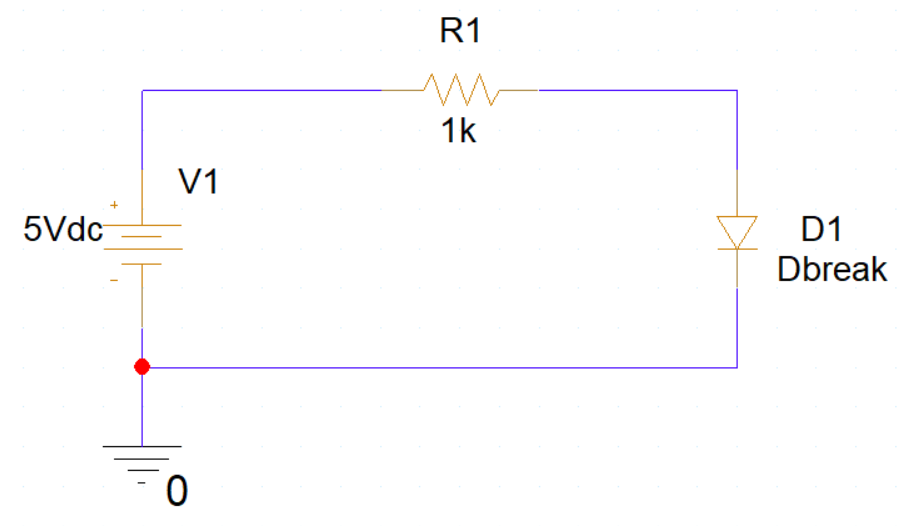
\includegraphics[width=4in]{source/picture/bai_2/diode_1.PNG}
    \caption{\textit{A simple simulation circuit using Diode}}
    \label{bai2_pic02}
\end{figure}


\textbf{Step 1: } Students are proposed to create a new project in PSPICE. Please select on the option \textbf{Create a blank project}.\\

\textbf{Step 2: } From the list of \textbf{Favorites} devices, search the component named \textbf{Dbreak}, which is a popular diode in circuit. Other components such as VDC, Resistor and the Ground, which are already used in Lab 1, are also added to the project as well. Finally, set the voltage supple of V1 to \textbf{5Vdc}.\\

\textbf{Step 3: } Create a simulation project by clicking on the menu \textbf{PSpice, New Simulation Profile}. After the name of the simulation profile is given, following dialog is shown:

\begin{figure}[!htp]
    \centering
    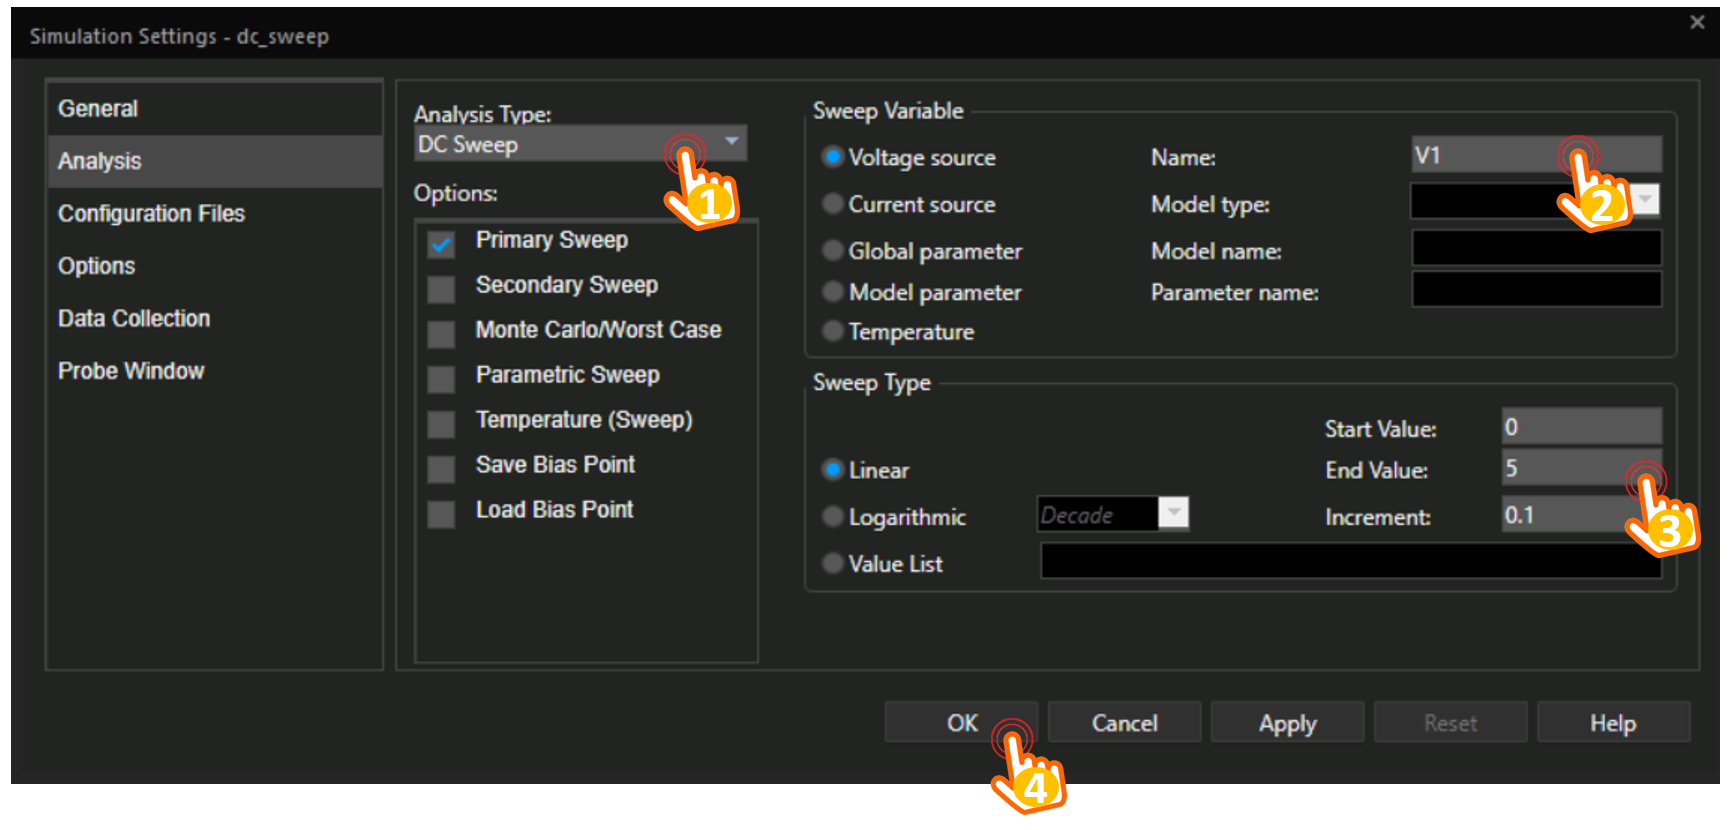
\includegraphics[width=4in]{source/picture/bai_2/diode_2.PNG}
    \caption{\textit{Configure the DC-Sweep simulation Profile}}
    \label{bai2_pic02_config}
\end{figure}


Following fields are required to configure:
\begin{itemize}
    \item \textbf{Analysis Type}: select \textbf{DC Sweep} mode
    \item \textbf{Sweep variable}: name of input source to analyze, which is (\textbf{V1}) in this case.
    \item \textbf{Sweep Type}: vary voltage of the source, which is from 0V to 5V and the incremental step is 0.1V.
\end{itemize}


\textbf{Step 5: } Run simulation (F11 or from menu \textbf{PSpice}, select \textbf{Run}). The simulation result for DC Sweep mode is launched as follows:

\begin{figure}[!htp]
    \centering
    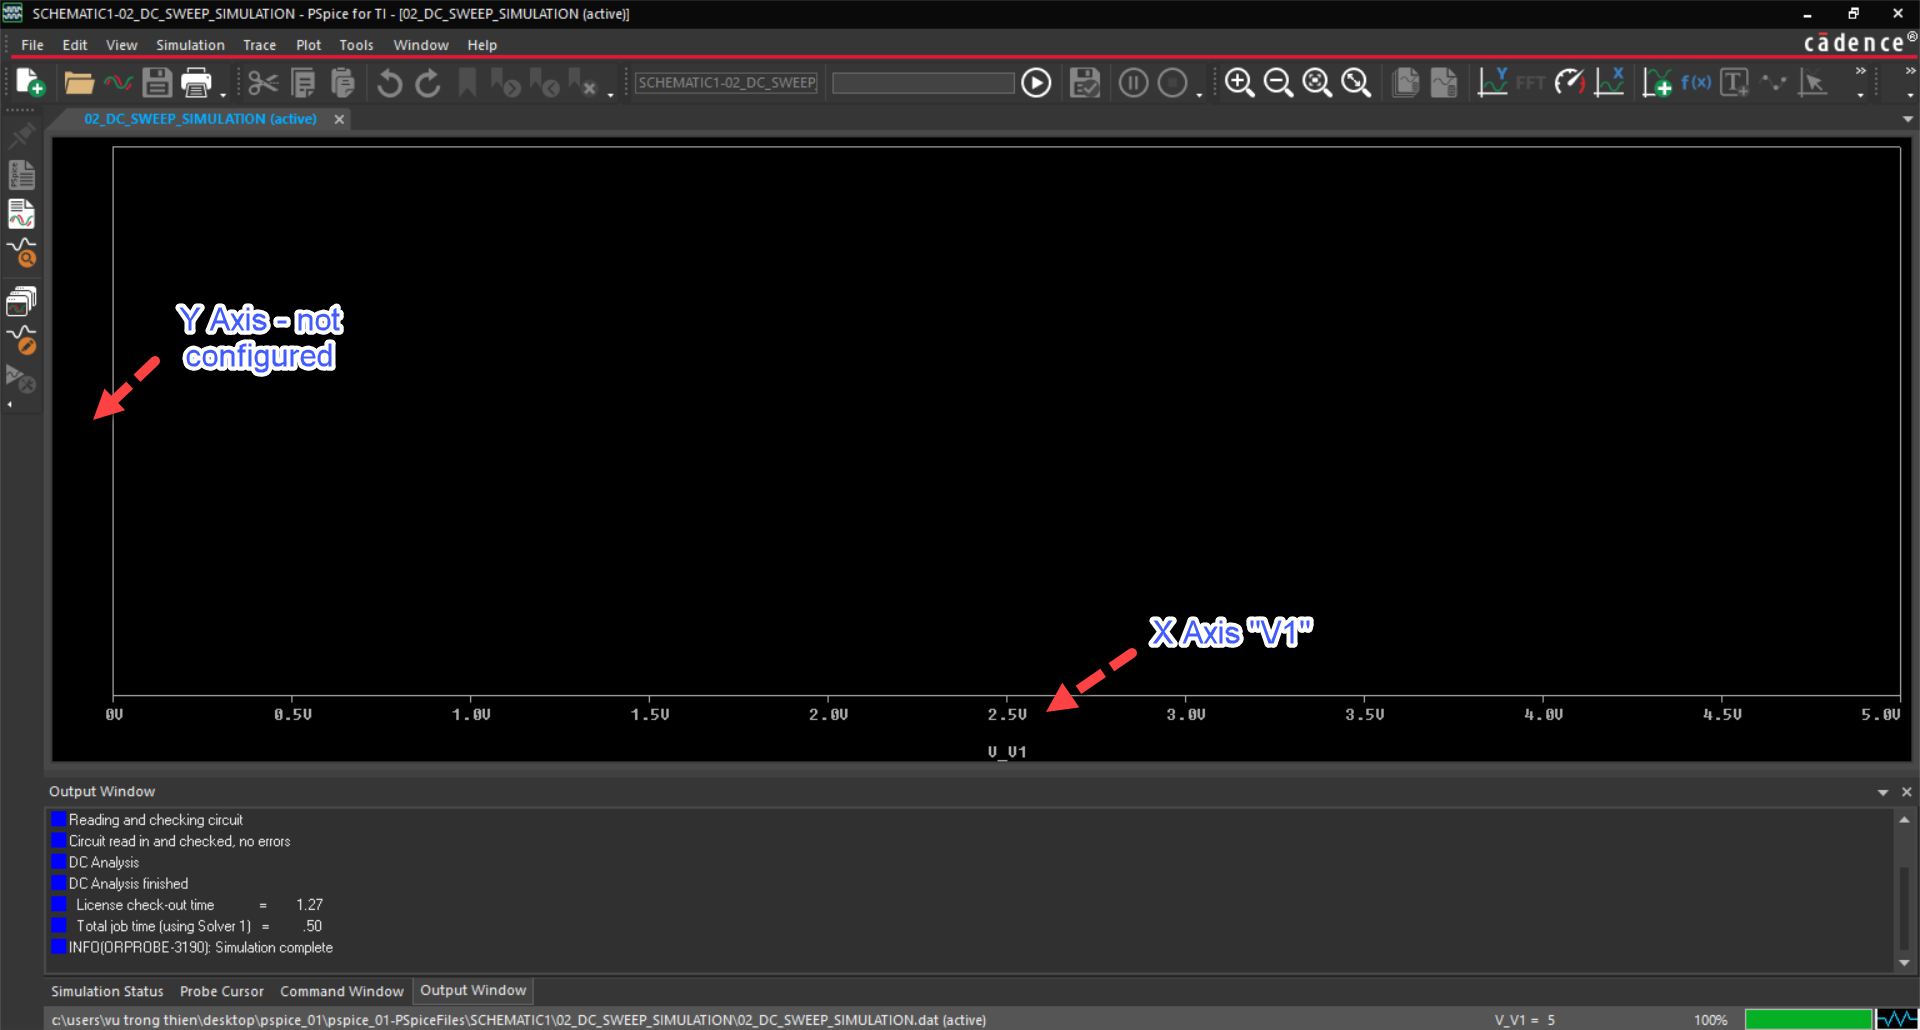
\includegraphics[width=4in]{source/picture/bai_2/12_RunSimulationNotConfigAxis.png}
    \caption{\textit{Simulation results for DC-Sweep mode}}
    \label{bai2_pic12}
\end{figure}

However, the screen is empty without any tracking information. In this case, we need to monitor the current in the circuit having a diode. To do this, from menu \textbf{Trace}, select \textbf{Add Trace} to open following dialog:

\begin{figure}[!htp]
    \centering
    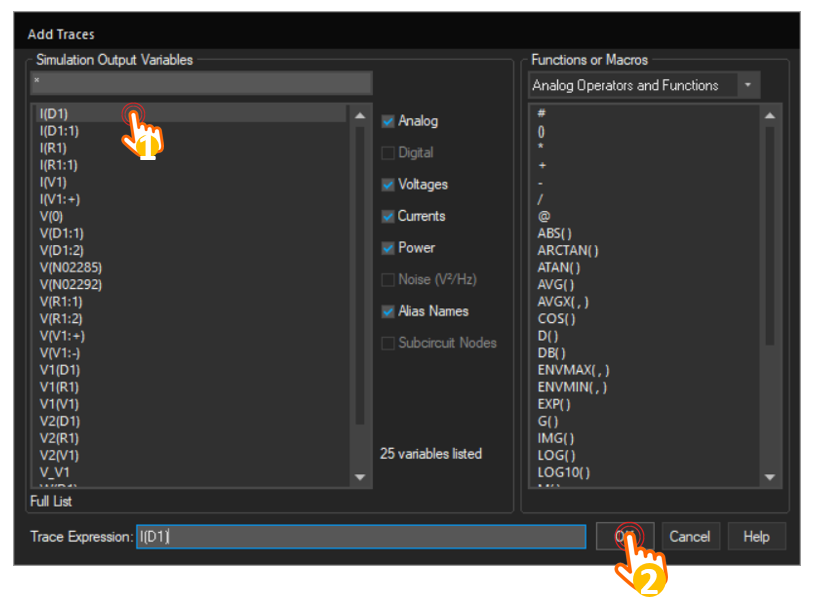
\includegraphics[width=4in]{source/picture/bai_2/14_ChooseID1ToYAxis.png}
    \caption{\textit{Add \textbf{I(D1)} to Y-Axis Trace}}
    \label{bai2_pic14}
\end{figure}

Choose \textbf{I(D1)} which is the current passing through the diode (and also the main current in the circuit having 2 components in a series). Finally, simulation results are depicted as follows:
\newpage
\begin{figure}[!htp]
    \centering
    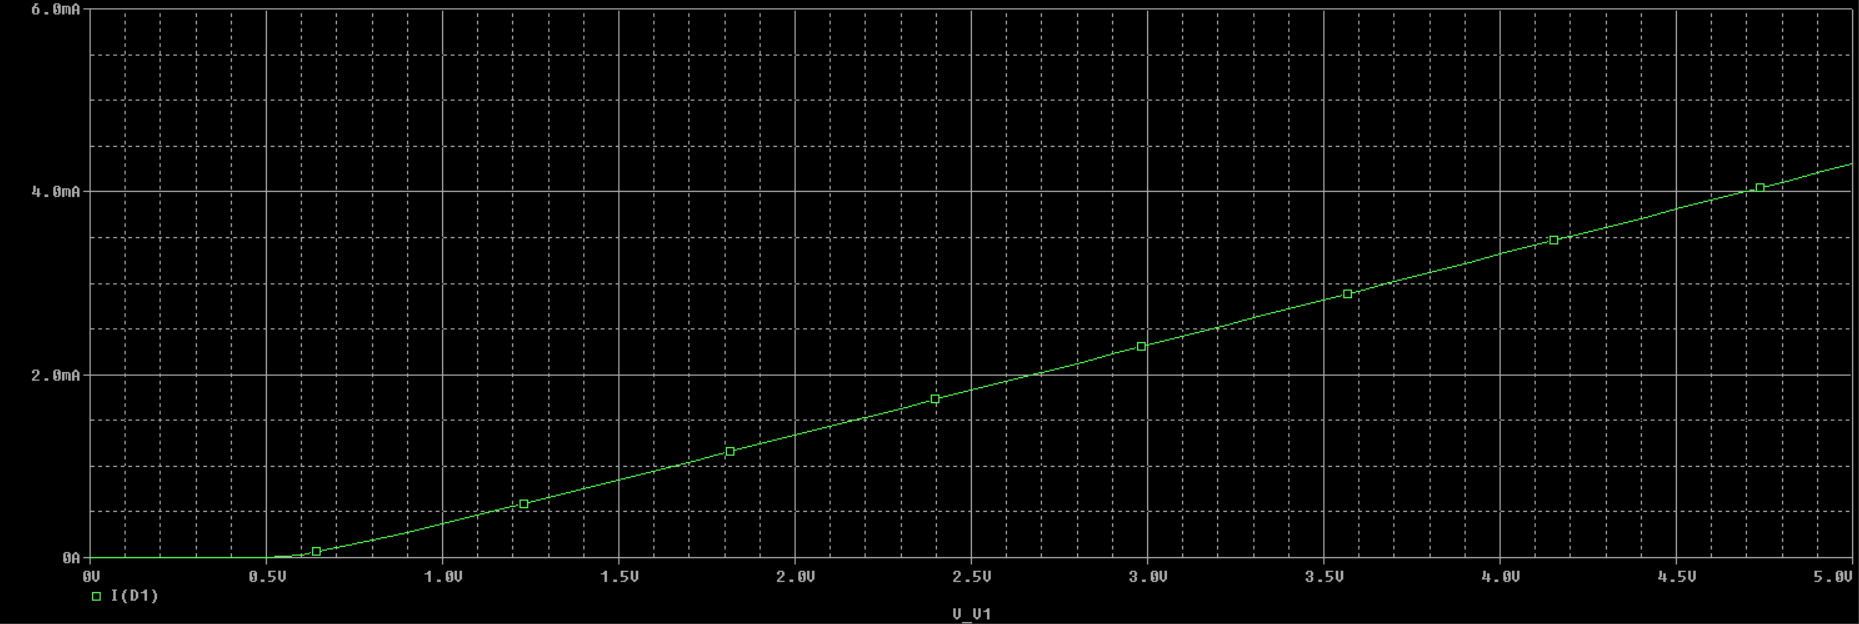
\includegraphics[width=5.5in]{source/picture/bai_2/15_ResultAfterAddYAxis.png}
    \caption{\textit{Simulation Result}}
    \label{bai2_pic15}
\end{figure}

\textbf{Step 6: } In order to make tracking information more readable, right click on the tracking line and choose \textbf{Trace Property} as follows:
\begin{figure}[!htp]
    \centering
    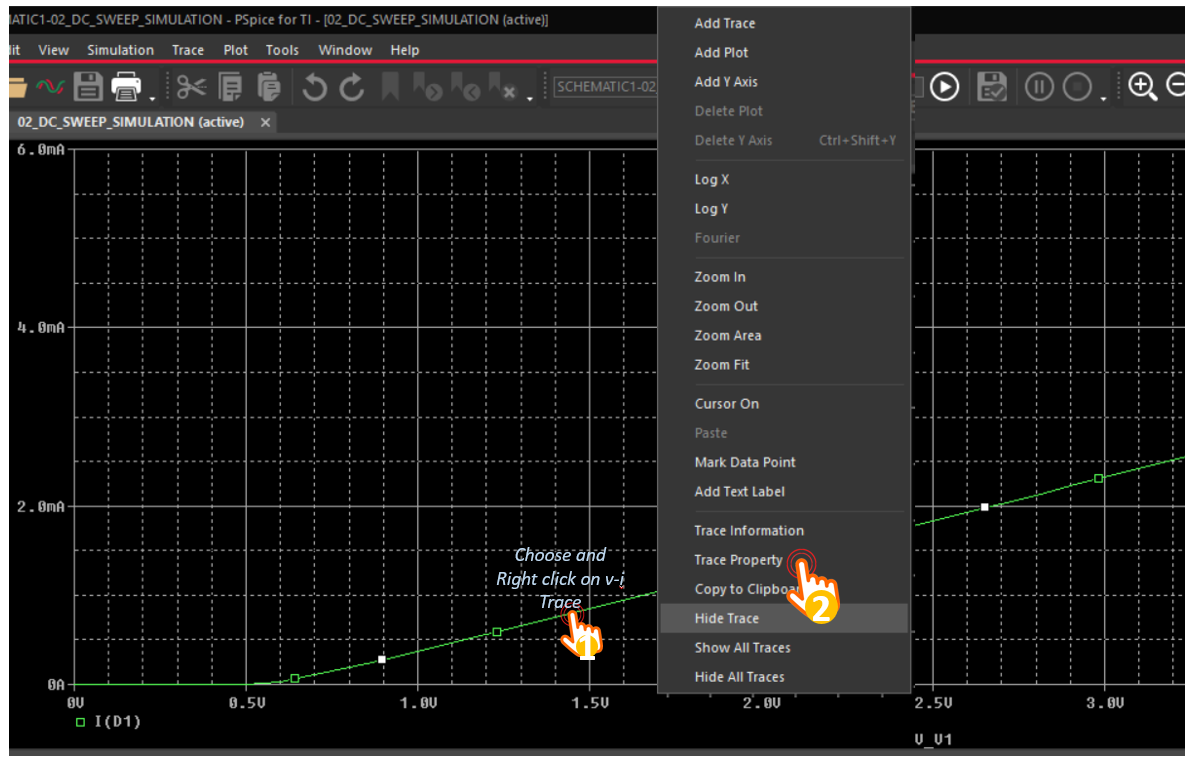
\includegraphics[width=4in]{source/picture/bai_2/16_ConfigTraceProperty.png}
    \caption{\textit{Configure Trace Property}}
    \label{bai2_pic16}
\end{figure}

The following dialog is opened, allow you to change the color and also the width of the tracking line

\begin{figure}[!htp]
    \centering
    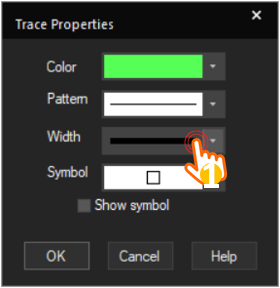
\includegraphics[width=2in]{source/picture/bai_2/17_ChangeWidthTrace.png}
    \caption{\textit{Change Trace Width to make it more readable}}
    \label{bai2_pic17}
\end{figure}
\newpage
The final shape of the simulation result is look like the following picture:

\begin{figure}[!htp]
    \centering
    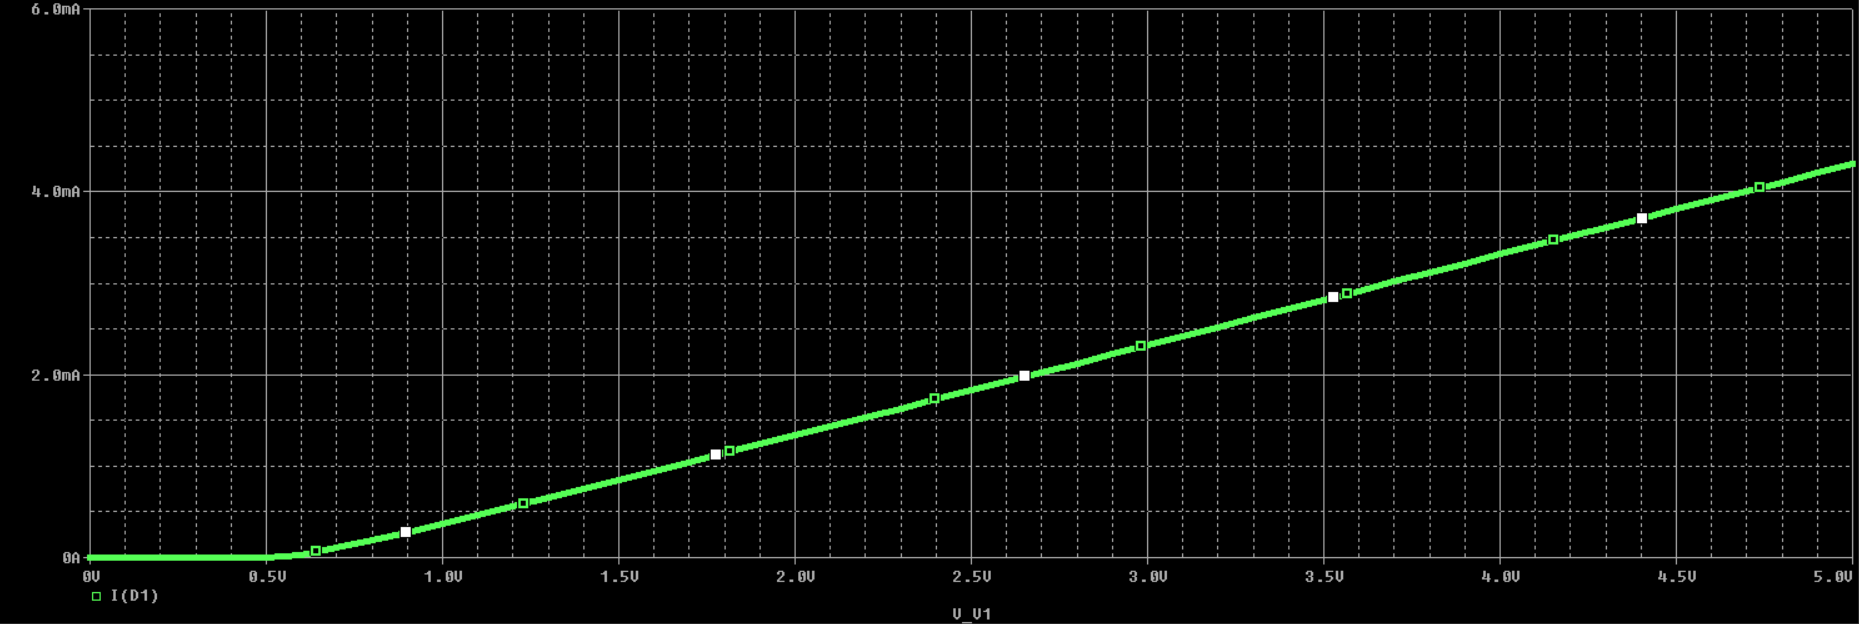
\includegraphics[width=5.5in]{source/picture/bai_2/18_ResultAfterConfigTrace.png}
    \caption{\textit{Simulation result after changing the Trace Width}}
    \label{bai2_pic18}
\end{figure}

The whole data for every point of the input voltage can be extract to text file by right click on the curve and select the option \textbf{Copy to Clipboard}. Finally, the data can be pasted to text editor, for instance, Notepad IDE.

\begin{figure}[!htp]
    \centering
    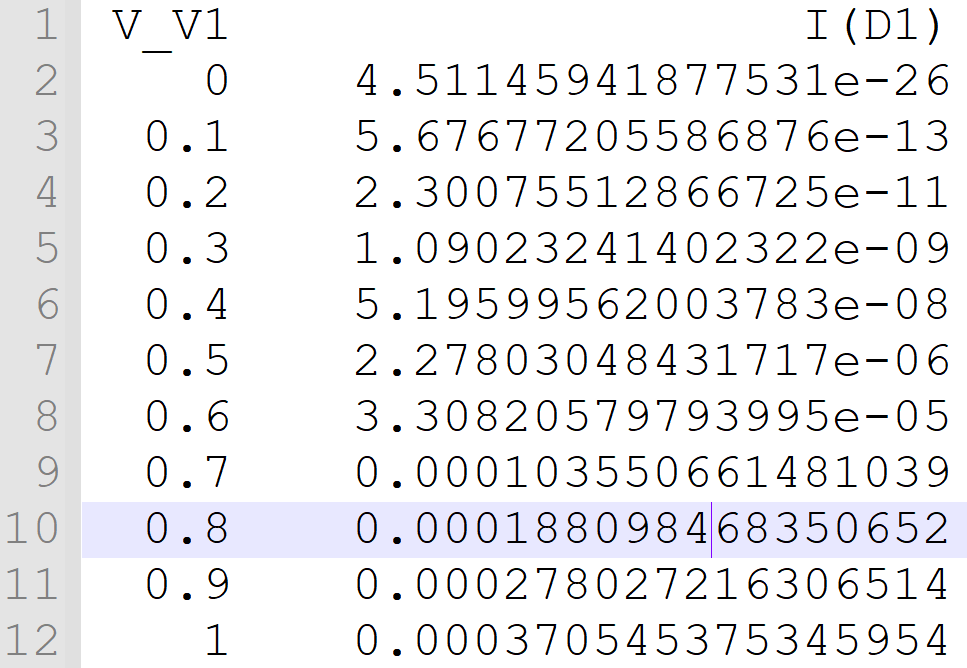
\includegraphics[width=3in]{source/picture/bai_2/diode_3.PNG}
    \caption{\textit{Extract data to Notepad Editor}}
    \label{bai2_pic18a}
\end{figure}

It is obviously that when the power supply is less than 0.7V, the current is close to zero (in order of $10^{-9}$ at 0.3V). However, when the input voltage is 1V, the current in the circuit is around 0.37mA. This result can be estimated as \textbf{(1V-0.7V)/1k}, when the practical diode model is applied. Students are proposed to check the simulation results at other points, such as V1 = 2V or V1 = 4V.\\


\textbf{Step 7: } A very important analysis with a diode is the relation between the voltage and the current across the diode, which is popular known as the V-I characteristic of the diode. To do this, on the simulation result windows, \textbf{double click on the X-Axis} to open the dialog as following:
\newpage
\begin{figure}[!htp]
    \centering
    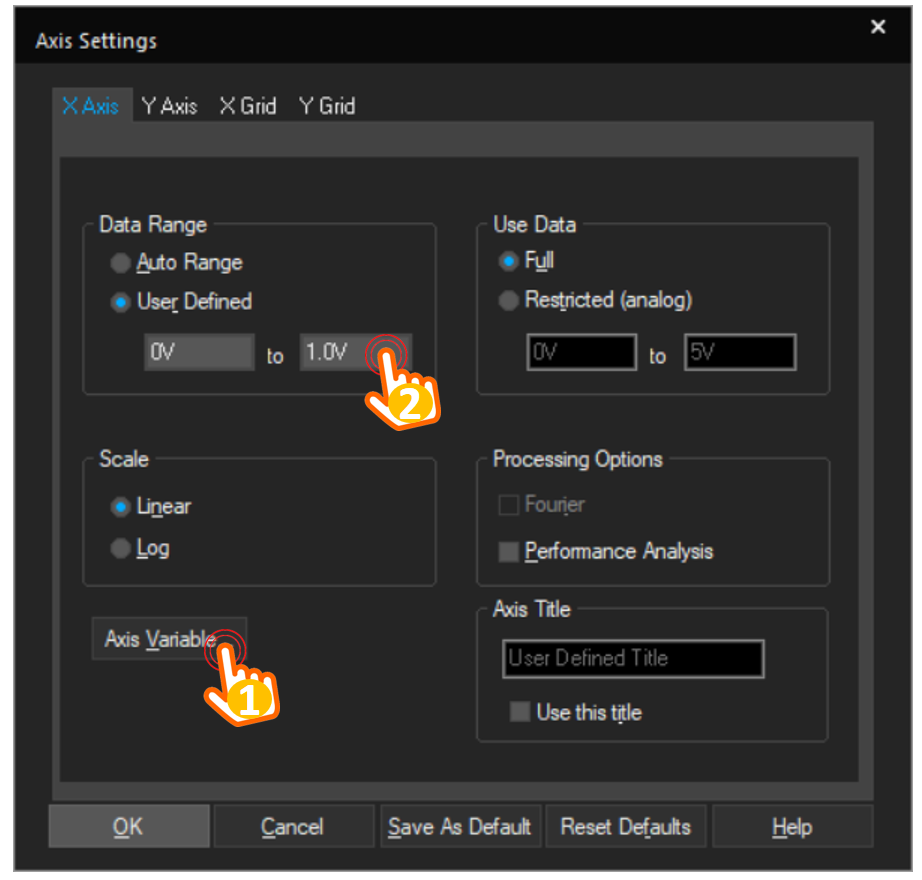
\includegraphics[width=4in]{source/picture/bai_2/diode_14.PNG}
    \caption{\textit{Set the X-Axis of the simulation result}}
    \label{bai2_pic18b}
\end{figure}

Firstly, clicking on the \textbf{Add Variables} button and select \textbf{V(D1:1)}, which is the voltage across the diode. Secondly, on the data range, \textbf{select from 0V to 1V in the User Defined} option. Finally, add a trace from menu Trace, and select I(D1) as previous simulation. The figure bellow is achieved:

\begin{figure}[!htp]
    \centering
    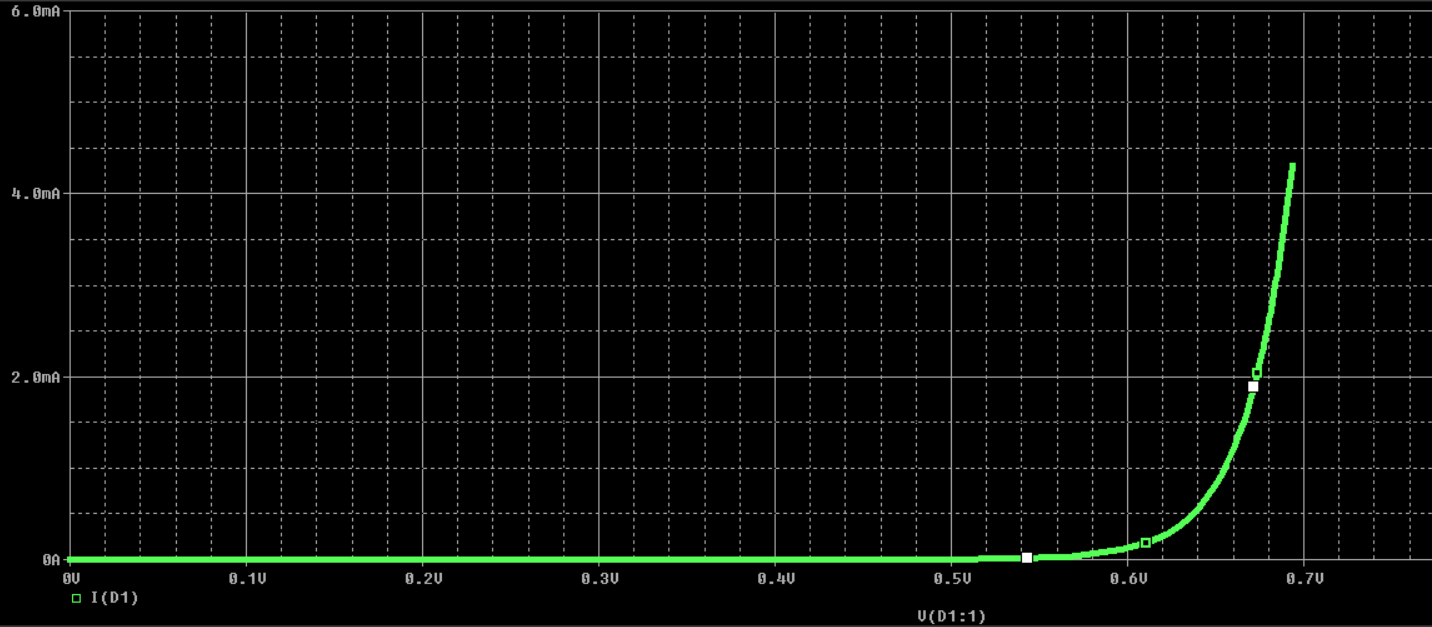
\includegraphics[width=5.5in]{source/picture/bai_2/diode_15.PNG}
    \caption{\textit{V-I characteristic of a diode}}
    \label{bai2_pic18c}
\end{figure}

This figure confirms that in the forward bias mode, the drop-down voltage of a diode is around 0.7V, which is the default value in the practical diode model.

\textbf{Step 8: } The bias simulation is also applied in this lab. By clicking on menu \textbf{PSpice, New Simulation Profile}. Similar to the first lab, after providing the name for the simulation profile(e.g. bias\_point), only the analysis type is changed to \textbf{Bias Point}. Finally, click \textbf{OK} button to create the second simulation profile.
\newpage
\begin{figure}[!htp]
    \centering
    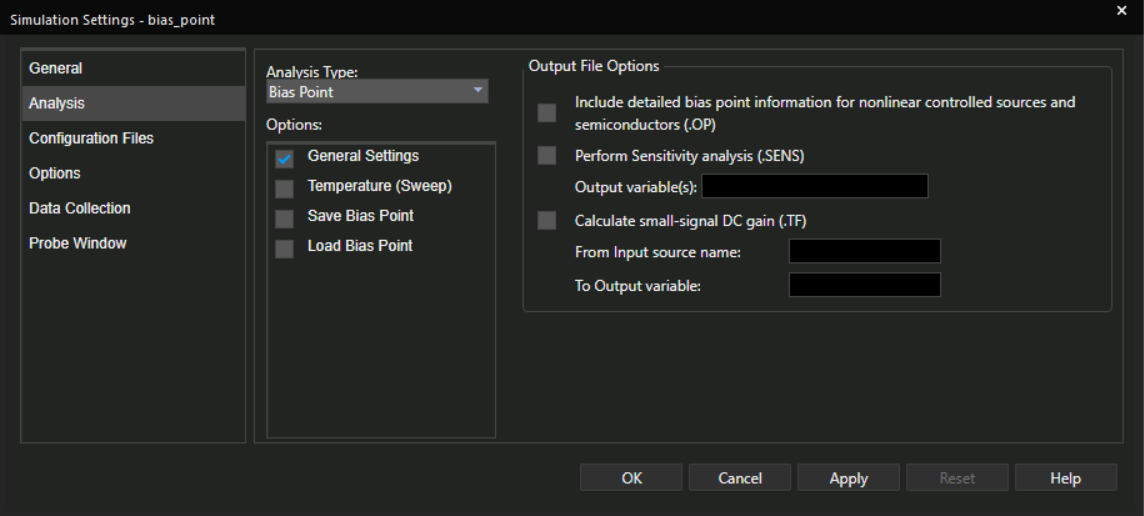
\includegraphics[width=4in]{source/picture/bai_2/diode_4.PNG}
    \caption{\textit{Add Bias Point simulation profile to the project}}
    \label{bai2_pic18d}
\end{figure}

Currently, there are two simulation profiles in the project, which can be browsed as following. In order to set a profile to active, right click on this profile and select \textbf{Make Active}.

\begin{figure}[!htp]
    \centering
    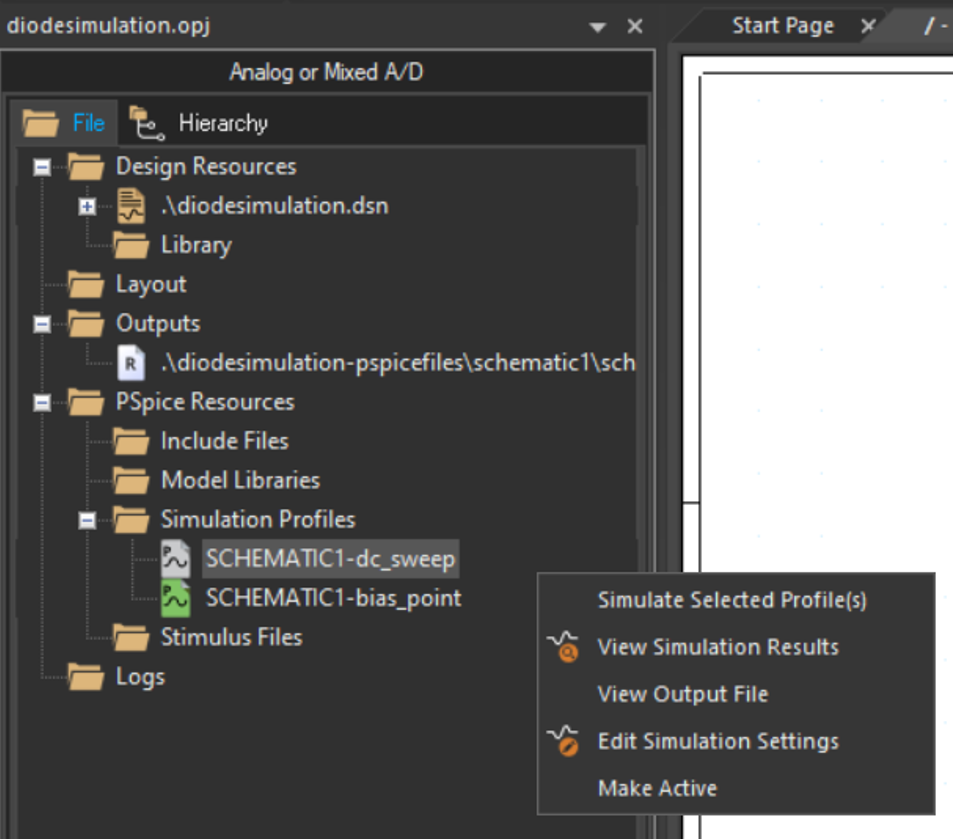
\includegraphics[width=3in]{source/picture/bai_2/diode_5.PNG}
    \caption{\textit{Set the active simulation profile}}
    \label{bai2_pic18e}
\end{figure}

Bias simulation results are displayed as follows:

\begin{figure}[!htp]
    \centering
    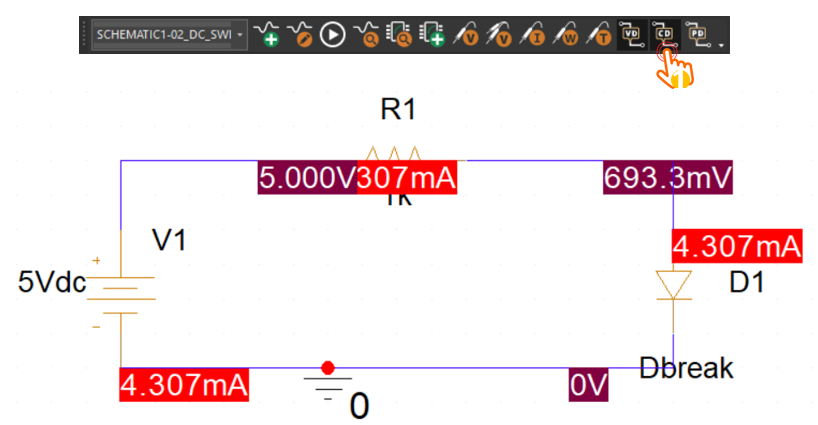
\includegraphics[width=4in]{source/picture/bai_2/21_EnableBiasCurrentDisplay.png}
    \caption{\textit{Enable Bias Current Display}}
    \label{bai2_pic21}
\end{figure}

From the simulation results, it is confirmed that the drop-down voltage of a diode is around 0.7V, which is very closed to the practical diode model.


\newpage
\section{Exercise and Report}
% Exercise 1: try above simulation circuit with other value of resistor to check voltage and current on circuit.
\subsection{Complete diode model}
According to the above simulation circuit (Figure 1.2), determine the voltage across the resistor and the diode ($V_{R}$, $V_{D}$), and also the current $I$ in the circuit with \textbf{two different values of R1}, including \textbf{220 Ohm} and \textbf{1.5K Ohm}. It is assumed that the complete diode model is used to analyse, having the forward voltage at \textbf{0.7V} and the internal resistor equal to \textbf{50 Ohm}.\\

Finally, the simulation on PSpice is run to double check with theory calculation. Brief explanations concerning the difference between theory and simulations can be provided in the report.\\

\subsubsection{Theory calculation}
\textit{\textbf{Notes:}}\\
\textit{Explanations, formulas, and equations are expected rather than only results.}\\

According to the: Ohm's Law and Complete diode model formula\bigskip\\
We have $V_{D}$: $V_D = I \cdot R_D + 0.7$\bigskip\\
Formula to calculate $V_{R}$: $ V_R = I \cdot R $\bigskip\\
Formula to calculate $I$: $I = \frac{V - 0.7}{R + r'_d}$\bigskip\\
Finally, when R = 220 Ohm, $V_{R} = I_{220} \cdot R = \frac{5-0.7}{220 + 50} \times 220 \approx 3.5037 (V)$ \bigskip\\
And when R = 1.5K Ohm, $V_{R} = I_{1.5K}\cdot R =\frac{5-0.7}{1500+50} \times 1500 \approx 4.16129 (V)$ \bigskip\\


\subsubsection{PSpice Simulation}
Set the simulation profile to bias-point. Moreover, enable both \textbf{Enable Voltage Bias Display} and \textbf{Enable Current Bias Display} to show the simulation results. \\

Students are supposed to capture the screen in PSPice and present in this report.

\textit{\textbf{Simulation results (images)}}:\\ \textit{Your image goes here}
\begin{figure}[!htp]
    \centering
    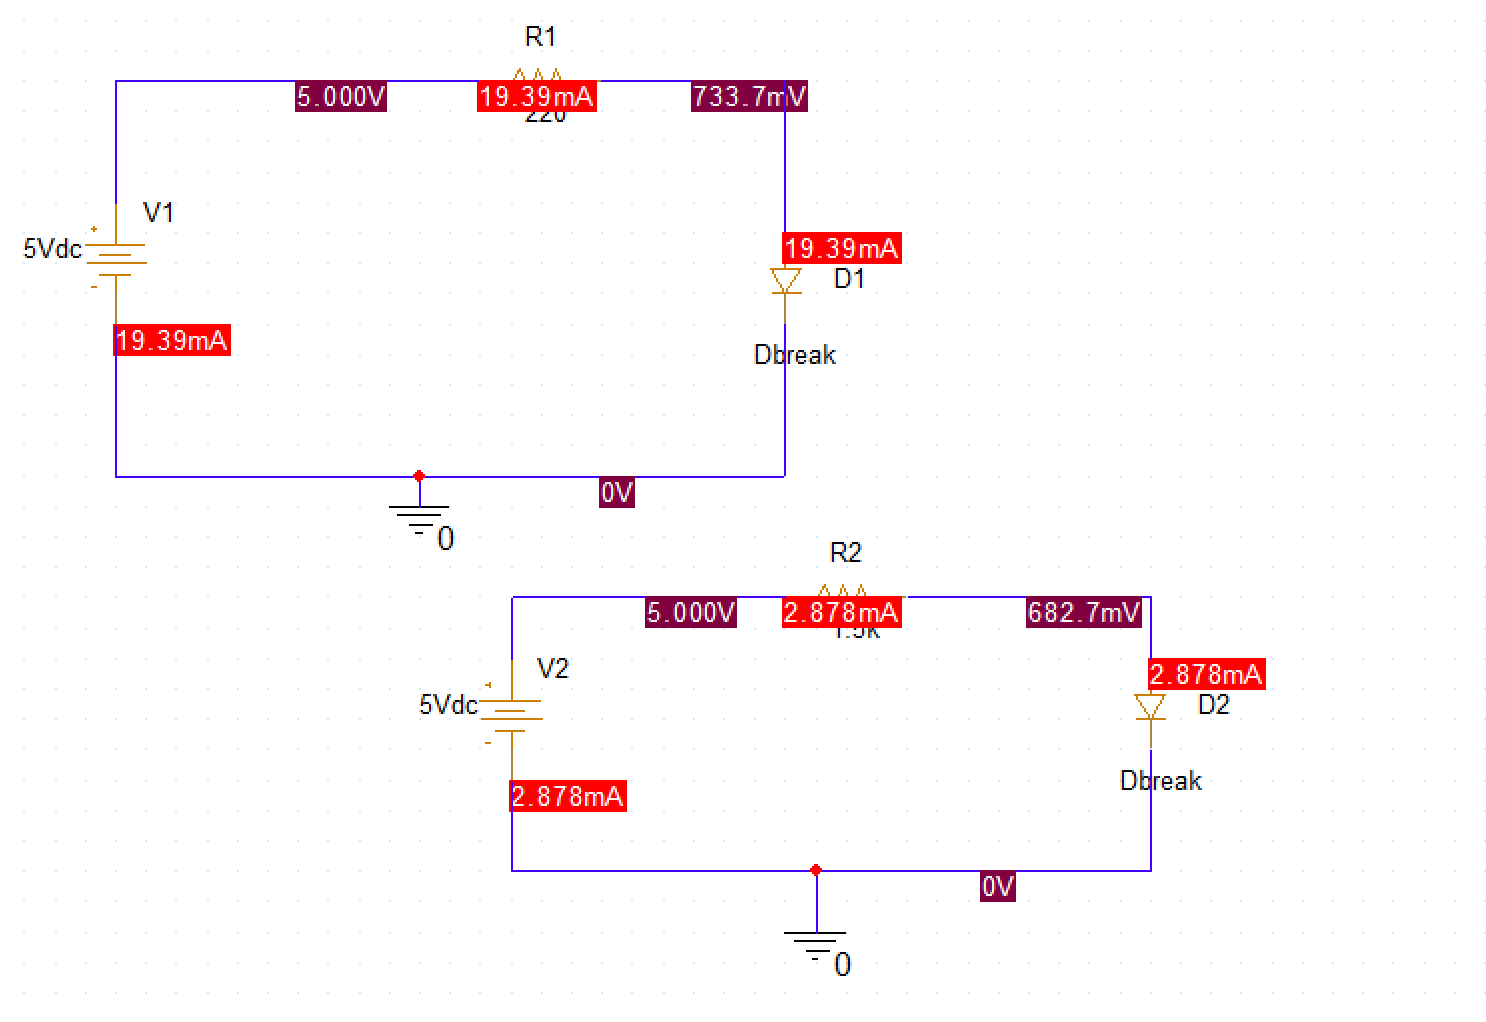
\includegraphics[width = 500px]{source/picture/bai_2/sim_ex1.png}
\end{figure}
\newpage

\subsubsection{Comparison}
In this section, the theory calculations and PSpice simulations are summarized in the table bellow to compare the difference. Students are supposed to fill all information in the table.
\begin{center}
    \begin{tabular}{l|l|l|l|l|l|l|}
        \cline{2-7}
                                          & \multicolumn{3}{c|}{\textbf{Theory}} & \multicolumn{3}{c|}{\textbf{PSpice}}                                                              \\ \cline{2-7}
                                          & $V_R$                                & $V_D$                                & I                     & $V_R$ & V & I                      \\ \hline
        \multicolumn{1}{|l|}{R = 220 Ohm} & 3.5037                               & 1.4963                               & 0.0159                &       &   & 0.01939                \\ \hline
        \multicolumn{1}{|l|}{R= 1.5K Ohm} & 4.1613                               & 0.8387                               & $2.77 \times 10^{-3}$ &       &   & $2.878 \times 10^{-3}$ \\ \hline
    \end{tabular}
\end{center}


According to the above \textbf{Exercise Results}, give some comments about observation (between calculation results and simulation results):\dotfill\bigskip
\dotfill\bigskip\par\mbox{}\dotfill
\dotfill\bigskip\par\mbox{}\dotfill
\dotfill\bigskip\par\mbox{}\dotfill
\dotfill\bigskip\par\mbox{}\dotfill

% Exercise 2: Diode Series
\subsection{Diode in a series}
Similar to the previous exercise, determine the value of the voltage $V_{D1}$, $V_{D2}$, $V_{D3}$ and the current $I$ for the give circuit. Then, simulate again the circuit using PSpice. However, in this case, the practical diode model is used with the forward voltage is 0.7223V.\\

\begin{figure}[!htp]
    \centering
    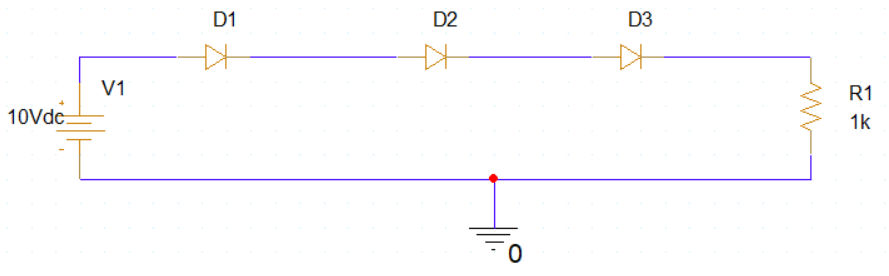
\includegraphics[width = 4in]{source/picture/bai_2/Lab02_Ex_02.png}
    \caption{Find the voltage and the current in the given circuit}
    \label{lab02_ex02}
\end{figure}


\subsubsection{Theory Calculation}
\textit{\textbf{Notes:}}\\
\textit{Explanations, formulas, and equations are expected rather than only results.}\\

According to the:\dotfill\bigskip\\
We have $V_{D1}$ =\dotfill\bigskip\\
$V_{D2}$ =\dotfill\bigskip\\
$V_{D3}$ =\dotfill\bigskip\\
$V_{R1}$ = \dotfill\bigskip\\
Formula to calculate $I$: \dotfill\bigskip\\
$I$ = \dotfill\bigskip\\



\subsubsection{PSpice Simulation}
Set the simulation profile to bias-point. Moreover, enable both \textbf{Enable Voltage Bias Display} and \textbf{Enable Current Bias Display} to show the simulation results. \\

Students are supposed to capture the screen in PSPice and present in this report.

\textit{\textbf{Simulation results (images):}} \textit{Your image goes here}\\
\begin{figure}[!htp]
    \centering
    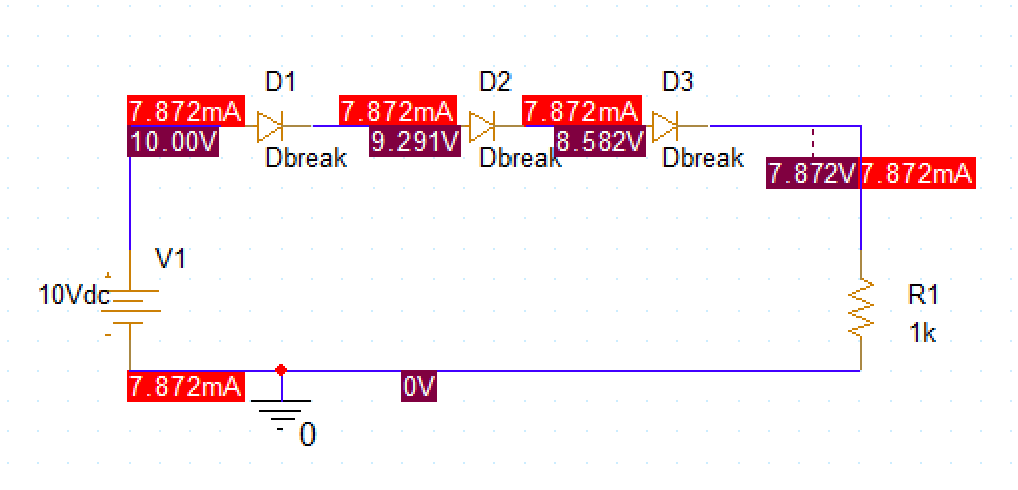
\includegraphics[width = 500px]{source/picture/bai_2/sim_ex2.png}
\end{figure}

\vspace{6cm}

\subsubsection{Comparison}

\begin{center}
    \begin{tabular}{l|l|l|l|l|l|}
        \cline{2-6}
                                          & \multicolumn{1}{c|}{$V_{D1}$} & \multicolumn{1}{c|}{$V_{D2}$} & \multicolumn{1}{c|}{$V_{D3}$} & \multicolumn{1}{c|}{$V_{R1}$} & \multicolumn{1}{c|}{$I$} \\ \hline
        \multicolumn{1}{|l|}{Calculation} & 0.7223V                       & 0.7223V                       & 0.7223V                       & 7.8331V                       & 7.8331mA                 \\ \hline
        \multicolumn{1}{|l|}{PSpice}      & 0.709V                        & 0.709V                        & 0.709V                        & 7.873V                        & 7.873mA                  \\ \hline
    \end{tabular}
\end{center}

The circuit in this exercise is a simple solution to design a power supply by leveraging a voltage drop of a diode. For example, a SIM module used to send SMS messages has a good voltage supply at 4.3V. In this case, a diode is connected from a 5V supply (which is a very popular voltage) and then, connected to the module SIM. Not only used to protect the module to avoid reverse current, a diode is a low-cost solution to generate 4.3V power supply for the SIM module.

\subsection{Circuit Analysis with Diode}
In PSpice, some exercise in the lesson can be simulated to confirm the results. Although it is not exactly the same values (e.g. voltage and current), the simulation in PSpice is a tool to check your solution. An example simulation circuit having diode and resistors is depicted as follows:

\begin{figure}[!htp]
    \label{pic:halfwave_rectifier3}
    \centering
    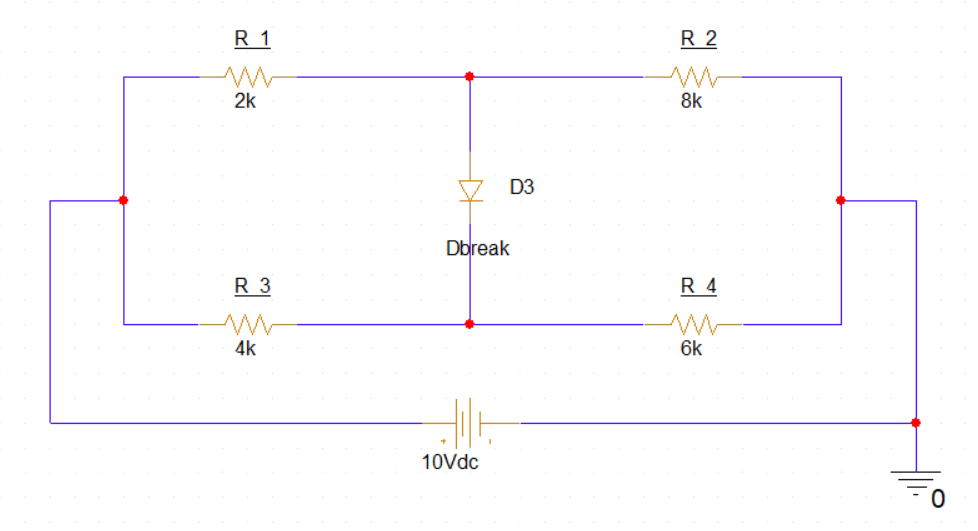
\includegraphics[width = 4in]{source/picture/bai_2/diode_10.PNG}
    \caption{Circuit analysis with diode}
    \label{lab02_ex031b}
\end{figure}

Students are proposed to analyse this circuit using practical diode model, with the drop-down voltage is around 0.7V. Then the simulation is run on PSpice to double check with your results.
\subsubsection{Theory calculation}
It is assumed that the voltage at anode and cathode of the diode $V_1$ and $V_2$. It is assumed that the diode is in forward bias mode.\\

According to the practical diode mode: $V_1$ -$V_2$ = 0.7V\\

Students are proposed to construct the equations to determine the current across all the resistors.

\dotfill\bigskip\par\mbox{}\dotfill
\dotfill\bigskip\par\mbox{}\dotfill
\dotfill\bigskip\par\mbox{}\dotfill
\dotfill\bigskip\par\mbox{}\dotfill
\subsubsection{PSpice simulation}
The bias point profile is used to run the simulation in this exercise. Students are proposed to capture the screen on PSpice showing the current and the voltage in the circuit.\\

\textit{Your image(s) goes here}\\
\begin{figure}[!htp]
    \centering
    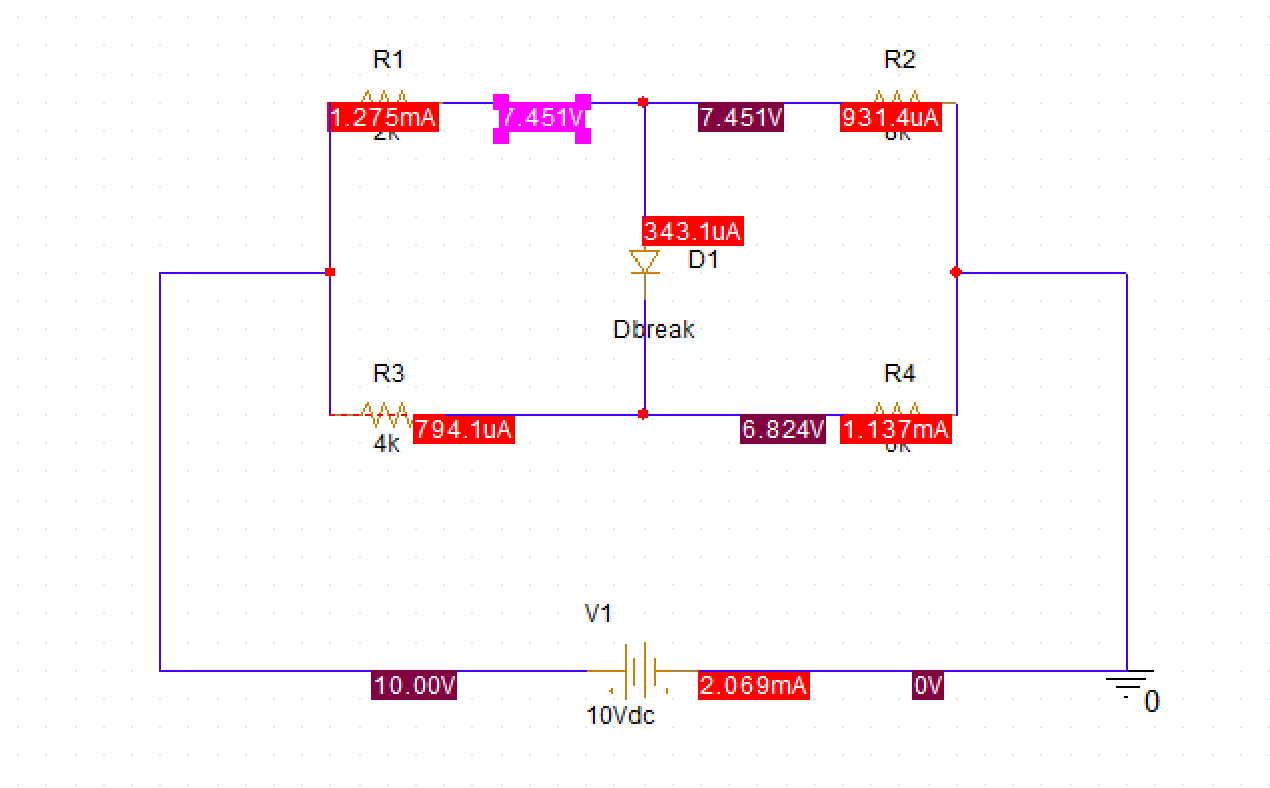
\includegraphics[width = 500px]{source/picture/bai_2/sim_ex3.png}
\end{figure}
\newpage
\subsubsection{Comparison}
Students are supposed to summarized the results from both theory calculations and PSpice simulations and fill in the table bellow.\\

\begin{center}

    \begin{tabular}{l|l|l|l|l|l|l|l|l|l|l|l|l|}
        \cline{2-13}
                                      & \multicolumn{6}{c|}{\textbf{Theory Calculation}} & \multicolumn{6}{c|}{\textbf{PSpice Simulation}}                                                                                                                                                                    \\ \cline{2-13}
                                      & \multicolumn{1}{c|}{$I_{R1}$}                    & \multicolumn{1}{c|}{$I_{R2}$}                   & \multicolumn{1}{c|}{$I_{R3}$} & \multicolumn{1}{c|}{$I_{R4}$} & \multicolumn{1}{c|}{$V_{1}$} & $V_2$ & $I_{R1}$ & $I_{R2}$ & $I_{R3}$ & $V_{R4}$ & $V_1$ & $V_2$ \\ \hline
        \multicolumn{1}{|l|}{V = 8V}  & 1.33                                             & 0.755                                           & 0.665                         & 0.89                          & 6.04                         & 5.34  & 0.996    & 0.751    & 0.653    & 0.898    & 6.008 & 5.389 \\ \hline
        \multicolumn{1}{|l|}{V = 12V} & 1.89                                             & 1.115                                           & 0.945                         & 1.37                          & 8,92                         & 8.22  & 1.553    & 1.112    & 0.395    & 1.377    & 8.894 & 8.260 \\ \hline
    \end{tabular}

\end{center}

\subsection{Clamper Diode Circuit}
The circuits in the figure below are known as clampers or DC restorers. The simulation on PSpice is also shown in the figure below. These circuits clamp a peak of a waveform to a specific DC level (e.g. 0.7V). Students are supposed to implement the circuit in PSPice to verify their results from therory calculation.
\\
\begin{figure}[!htp]
    \label{pic:halfwave_rectifier1}
    \centering
    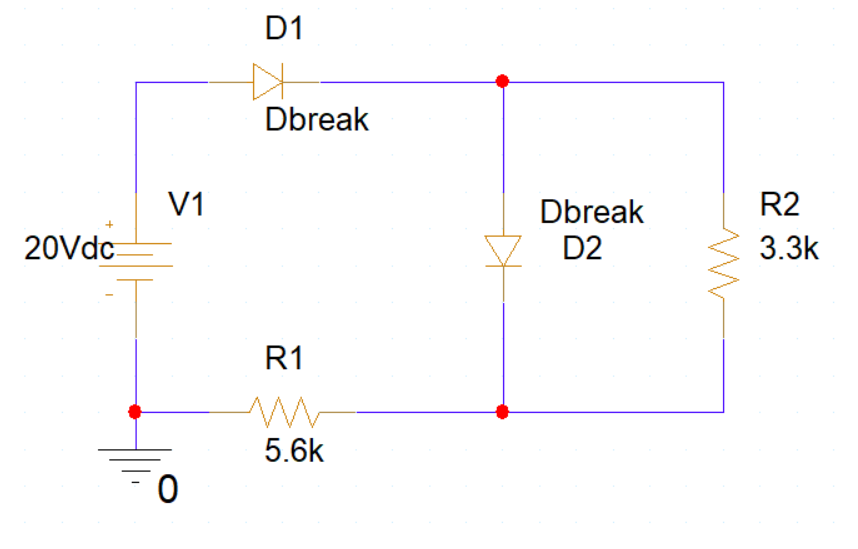
\includegraphics[width = 3.5in]{source/picture/bai_2/diode_11.PNG}
    \caption{Clamper circuit using diode}
    \label{lab02_ex031c}
\end{figure}

\subsubsection{Theory calculation}
In this part, it is assumed that the practical diode model is used. Present your equations to calculate three different currents, including $I_{R1}$, $I_{R2}$, $I_{D2}$ and the voltage $V_{R2}$.

\dotfill\bigskip\par\mbox{}\dotfill
\dotfill\bigskip\par\mbox{}\dotfill
\dotfill\bigskip\par\mbox{}\dotfill
\dotfill\bigskip\par\mbox{}\dotfill

\subsubsection{PSpice simulation}
The bias point simulation is run in PSpice. Capture your screen with voltage and current are enabled in the results.

\textit{Your image(s) goes here}\\
\begin{figure}[!htp]
    \centering
    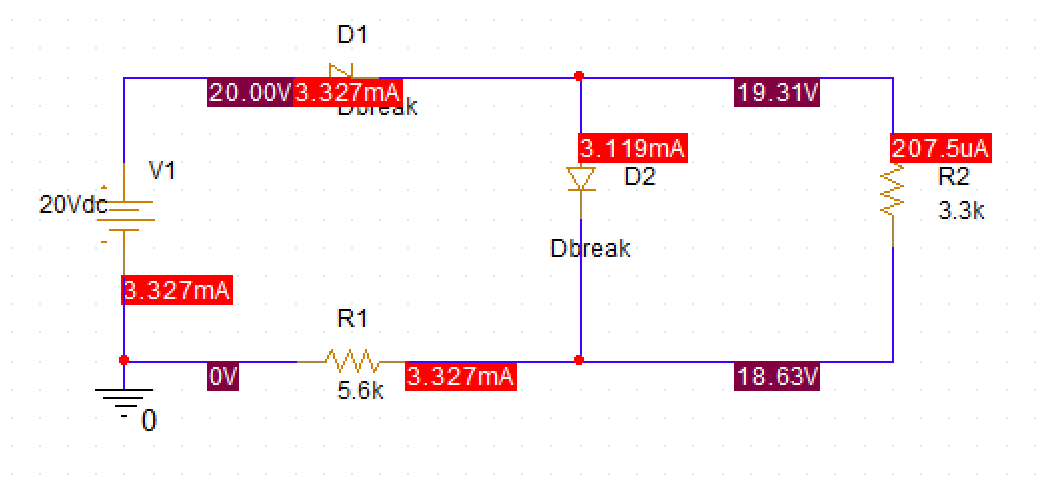
\includegraphics[width = 500px]{source/picture/bai_2/sim_ex4.png}
\end{figure}

\vspace{8cm}

\subsubsection{Comparison}

Students are supposed to summarized the results from both theory calculations and PSpice simulations and fill in the table bellow.\\

\begin{center}

    \begin{tabular}{l|l|l|l|l|l|l|l|l|}
        \cline{2-9}
                                      & \multicolumn{4}{c|}{Theory calculation} & \multicolumn{4}{c|}{PSpice simulation}                                                                                                             \\ \cline{2-9}
                                      & \multicolumn{1}{c|}{$I_{R1}$}           & \multicolumn{1}{c|}{$I_{R2}$}          & \multicolumn{1}{c|}{$I_{D2}$} & \multicolumn{1}{c|}{$V_{R2}$} & $I_{R1}$ & $I_{R2}$ & $I_{D2}$ & $V_{R2}$ \\ \hline
        \multicolumn{1}{|l|}{V = 12V} & 1.893                                   & 0.212                                  & 1.681                         & 0.7                           & 1.903    & 0.203    & 1.701    & 0.67     \\ \hline
        \multicolumn{1}{|l|}{V = 20V} & 3.321                                   & 0.212                                  & 3.109                         & 0.7                           & 3.327    & 0.208    & 3.119    & 0.68     \\ \hline
    \end{tabular}
\end{center}

What can be concluded from this table?

\subsection{Power switching circuit}

The corruption of main power can be crucial in many different situations. For instance, when power is abruptly lost, you might want to save some backup data on a micro-controller. Such use cases need some form of automatic switching circuit to a secondary power source, such as a battery.\\

\newpage

\begin{figure}[!htp]
    \label{pic:halfwave_rectifier2}
    \centering
    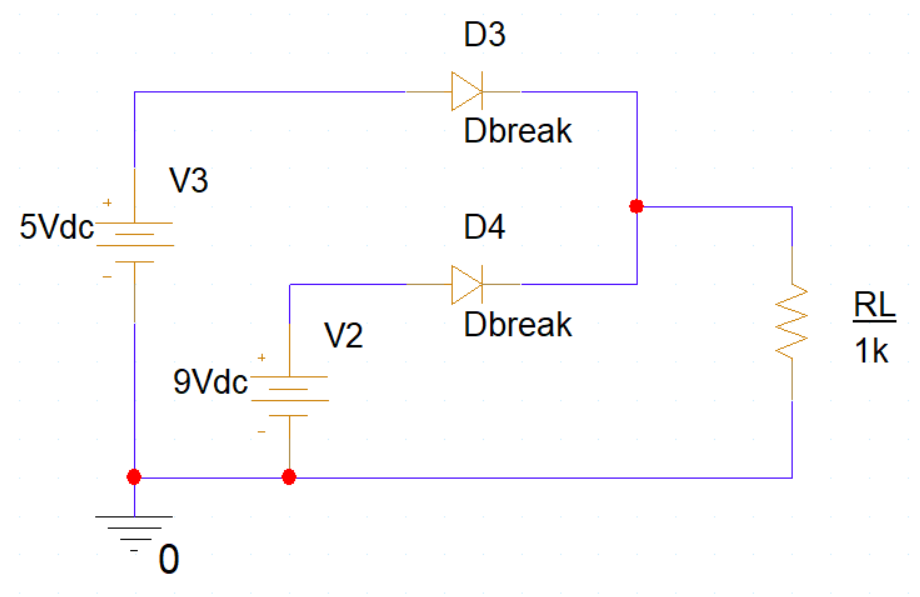
\includegraphics[width = 3.5in]{source/picture/bai_2/diode_12.PNG}
    \caption{Power switching circuit}
    \label{lab02_ex031d}
\end{figure}

The simplest solution to this problem is simply to add a diode on each voltage source, as shown in the figure above. In this circuit, a 5V power supply can be used as a backup battery. Meanwhile, 9V is the main power supply for the system, which is demonstrated by a load resistor.\\

However, the main issue with this naive approach is that the voltage drop (forward voltage) across the diode might be too high for the system. Thanks to Schottky diode, this can be mitigated by using extremely low forward voltage one, which can be found on the market (e.g. Schottky diode having drop-down voltage around 250mV at 1A).

\subsubsection{Theory calculation}
In this part, it is assumed that the practical diode model is used. Present your equations to calculate the current $I_{D3}$, $I_{D4}$, $I_{RL}$ and the volatage $V_{RL}$ in three different cases: only 5V, only 9V and both 5V and 9V for the power supply.\\

\dotfill\bigskip\par\mbox{}\dotfill
\dotfill\bigskip\par\mbox{}\dotfill
\dotfill\bigskip\par\mbox{}\dotfill
\dotfill\bigskip\par\mbox{}\dotfill

\subsubsection{PSpice simulation}
The bias point simulation is run in PSpice with both power sources are enabled. Capture your screen with voltage and current are enabled in the results.\\

\textit{Your image(s) goes here}
\begin{figure}[!htp]
    \centering
    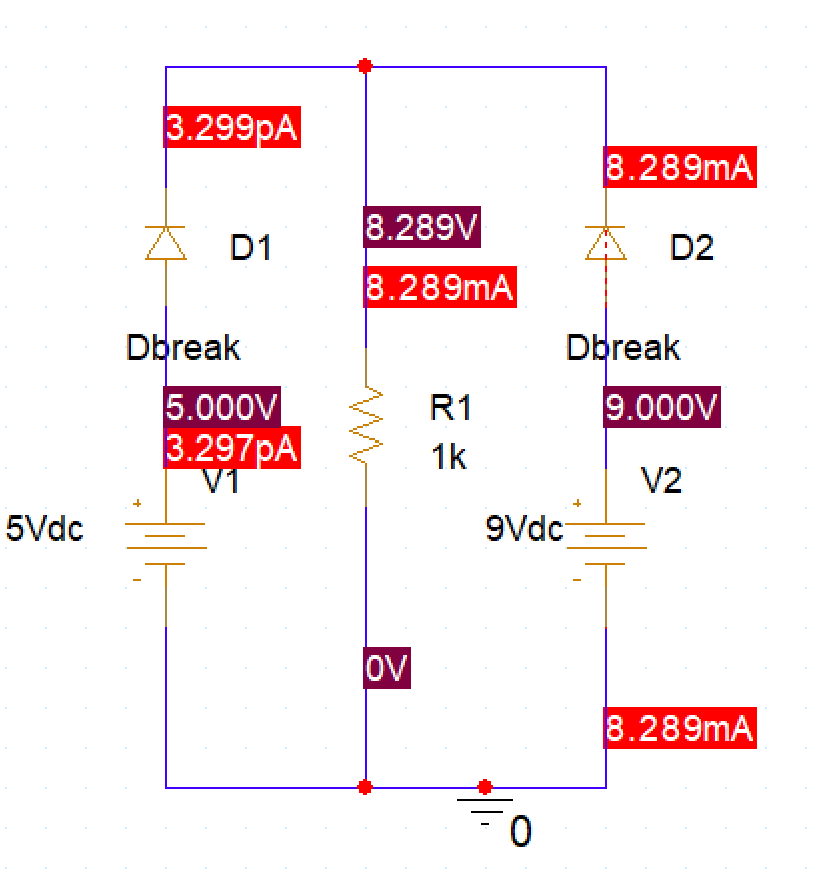
\includegraphics[width = 500px]{source/picture/bai_2/sim_ex5.png}
    \label{sim_ex5}
\end{figure}
\newpage
\vspace{8cm}

\subsubsection{Comparison}
Students are supposed to summarized the results from both theory calculations and PSpice simulations and fill in the table bellow. Both power sources are connected to the circuit.\\

\begin{center}
    \begin{tabular}{|l|l|l|l|l|l|l|l|}
        \hline
        \multicolumn{4}{|c|}{Theory calculation} & \multicolumn{4}{c|}{PSpice simulation}                                                                                                             \\ \hline
        \multicolumn{1}{|c|}{$I_{D1}$}           & \multicolumn{1}{c|}{$I_{D2}$}          & \multicolumn{1}{c|}{$I_{RL}$} & \multicolumn{1}{c|}{$V_{RL}$} & $I_{D1}$ & $I_{D2}$ & $I_{RL}$ & $V_{RL}$ \\ \hline
        0                                        & 8.3                                    & 8.3                           & 8.3                           & 3.299    & 8.289    & 8.289    & 8.289    \\ \hline
    \end{tabular}
\end{center}


The last feature of the diodes in this circuit is  to protect the reverse current in case both the power sources are switch on together. This use case is very popular when a micro-controller platform is programmed and powered by an USB port and also equipped with an adapter for external power supply.

% Exercise 3: Half-wave Rectifier.
% https://www.youtube.com/watch?v=A7pHAu2W5fE
\subsection{Half-wave Rectifier}
\label{halfwaveRectifier}
In this exercise, an alternating source is used to generate a half-wave rectifier output using a diode. The schematic of the simulation is given bellow:

\begin{figure}[!htp]
    \label{pic:halfwave_rectifier}
    \centering
    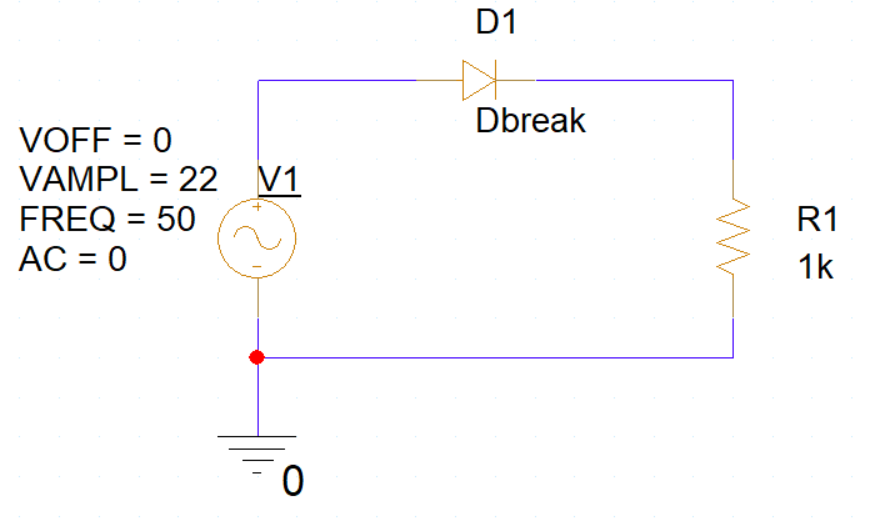
\includegraphics[width = 3.5in]{source/picture/bai_2/diode_6.PNG}
    \caption{Half-wave Rectifier with Voltage Sin Source}
    \label{lab02_ex031}
\end{figure}

\textbf{Step 1: } Create the schematic.\\
The new component in this schematic is the \textbf{VSIN - Sine Voltage Source}, which can be found in the Favorites list. This component has four different parameters are required to configure, as follows:
\begin{itemize}
    \item VOFF: Offset voltage of the source
    \item VAMPL: Amplifier voltage of the source
    \item FREQ: Frequency of the alternative current
    \item AC: The source type (having value 0 or 1), to switch between VAC and VSIN. In VSIN source, the frequency can be modified.
\end{itemize}

After setting these parameters are set to the values shown in the figure above, add a voltage probe to track the output by clicking on the \textbf{Voltage/Level Marker} on the PSpice Toolbar, as follows:

\begin{figure}[!htp]
    \label{pic:halfwave_rectifier4}
    \centering
    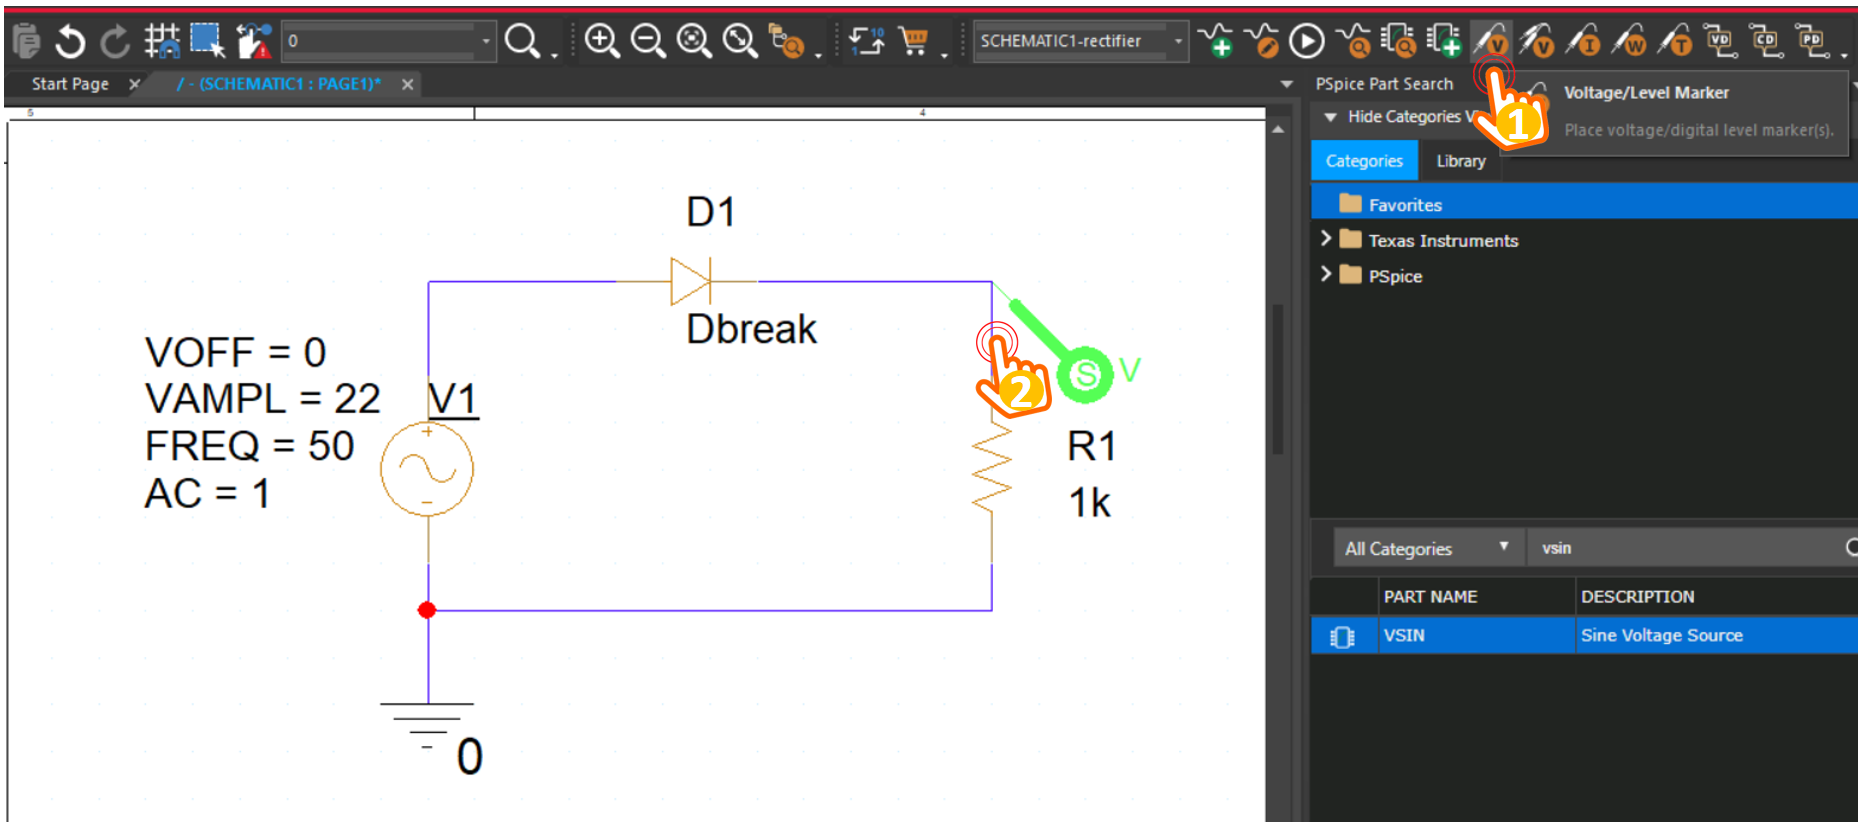
\includegraphics[width = 5in]{source/picture/bai_2/diode_7.PNG}
    \caption{Add a voltage marker for simulation tracing}
    \label{lab02_ex031f}
\end{figure}

\textbf{Step 2: } Create a new simulation profile.
In order to generate the output signal of the voltage probe, the analysis type is set to \textbf{Time Domain (Transient)}. Moreover, due to the frequency of the power source is 50Hz, the \textbf{simulation time is set to 100ms}, to depict 10 cycles of the output signal. Finally, the resolution is set to 0.1ms in the \textbf{Maximum Step size}. The configuration windows for this simulation profile is presented as follows:

\begin{figure}[!htp]
    \label{pic:halfwave_rectifier5}
    \centering
    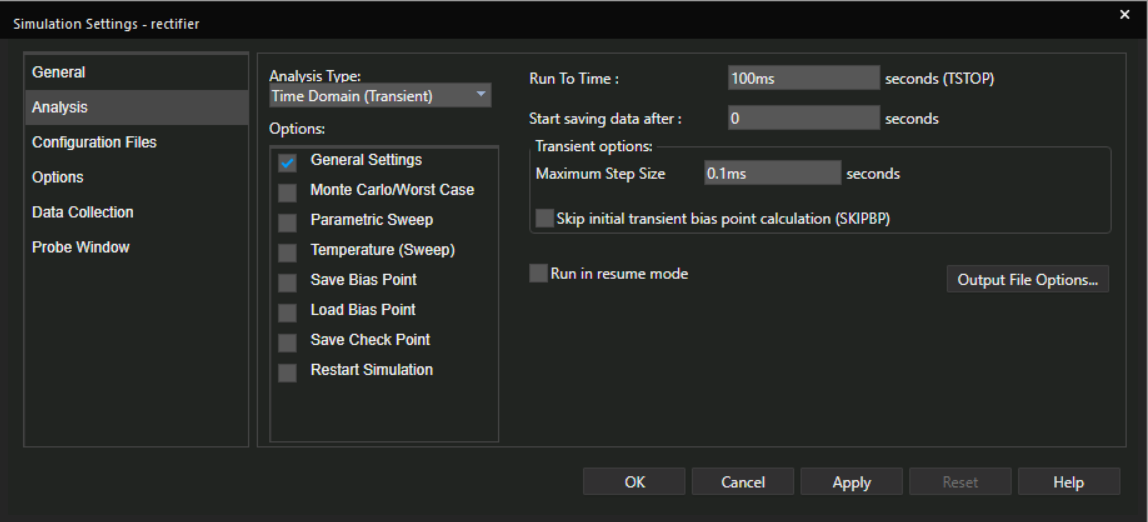
\includegraphics[width = 5in]{source/picture/bai_2/diode_8.PNG}
    \caption{Create Time Domain simulation profile}
    \label{lab02_ex031z}
\end{figure}


\textbf{Step 3: } Run the simulation and observe the results
Finally, run the simulation and the output on the simulation windows should be presented in  the figure bellow:

\begin{figure}[!htp]
    \label{pic:halfwave_rectifier6}
    \centering
    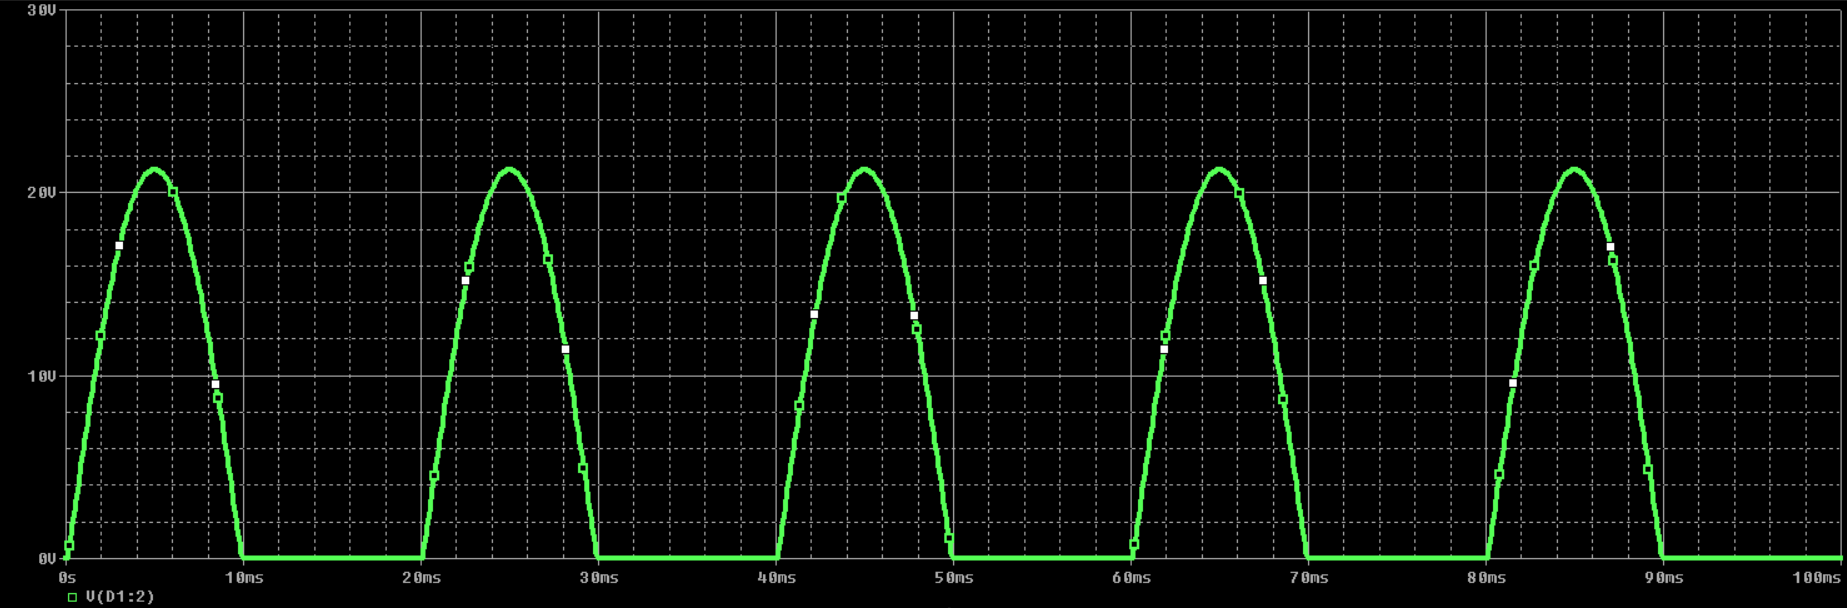
\includegraphics[width = 5in]{source/picture/bai_2/diode_9.PNG}
    \caption{Wave form for the half-ware rectifier circuit}
    \label{lab02_ex031h}
\end{figure}



\subsubsection{Theory calculation}
\textit{\textbf{Notes:}}\\
\textit{Explanations, formulas, and equations are expected rather than only results.}\\

\textbf{\textit{Approximation:}} Diodes have $V_f$ = 0.78V\\
\begin{itemize}
    \item Minimum Value of $V_{R1}$ = 0V \dotfill\\
    \item Maximum Value of $V_{R1} = V - V_D = 22 - 0.78 = 21.2628V$\dotfill\\
    \item Duration (millisecond) for a cycle of $V_{R1} = \frac{1}{f} = \frac{1}{50} = 20ms$ \dotfill\\
\end{itemize}

\subsubsection{PSpice simulation}
Export your simulation results to Notepad for instance, and find the minimum and the maximum point of the output voltage, then fill your answer to the section bellow:

\begin{itemize}
    \item Minimum Value of $V_{R1}$ = $-1.92756 \mu V$ \dotfill\\
    \item Maximum Value of $V_{R1} = V - V_D = 22 - 0.78 = 21.263V$ \dotfill\\
    \item Duration (millisecond) for a cycle of $V_{R1}$: $\frac{1}{f} = \frac{1}{50} = 20ms$ \dotfill\\
\end{itemize}

The tracking point can also be used directly on the simulation output windows, by the \textbf{Toggle Cursor} option on the toolbar. A Probe Cursor window is opened to update a tracking point.
\begin{figure}[!htp]
    \label{pic:halfwave_rectifier7}
    \centering
    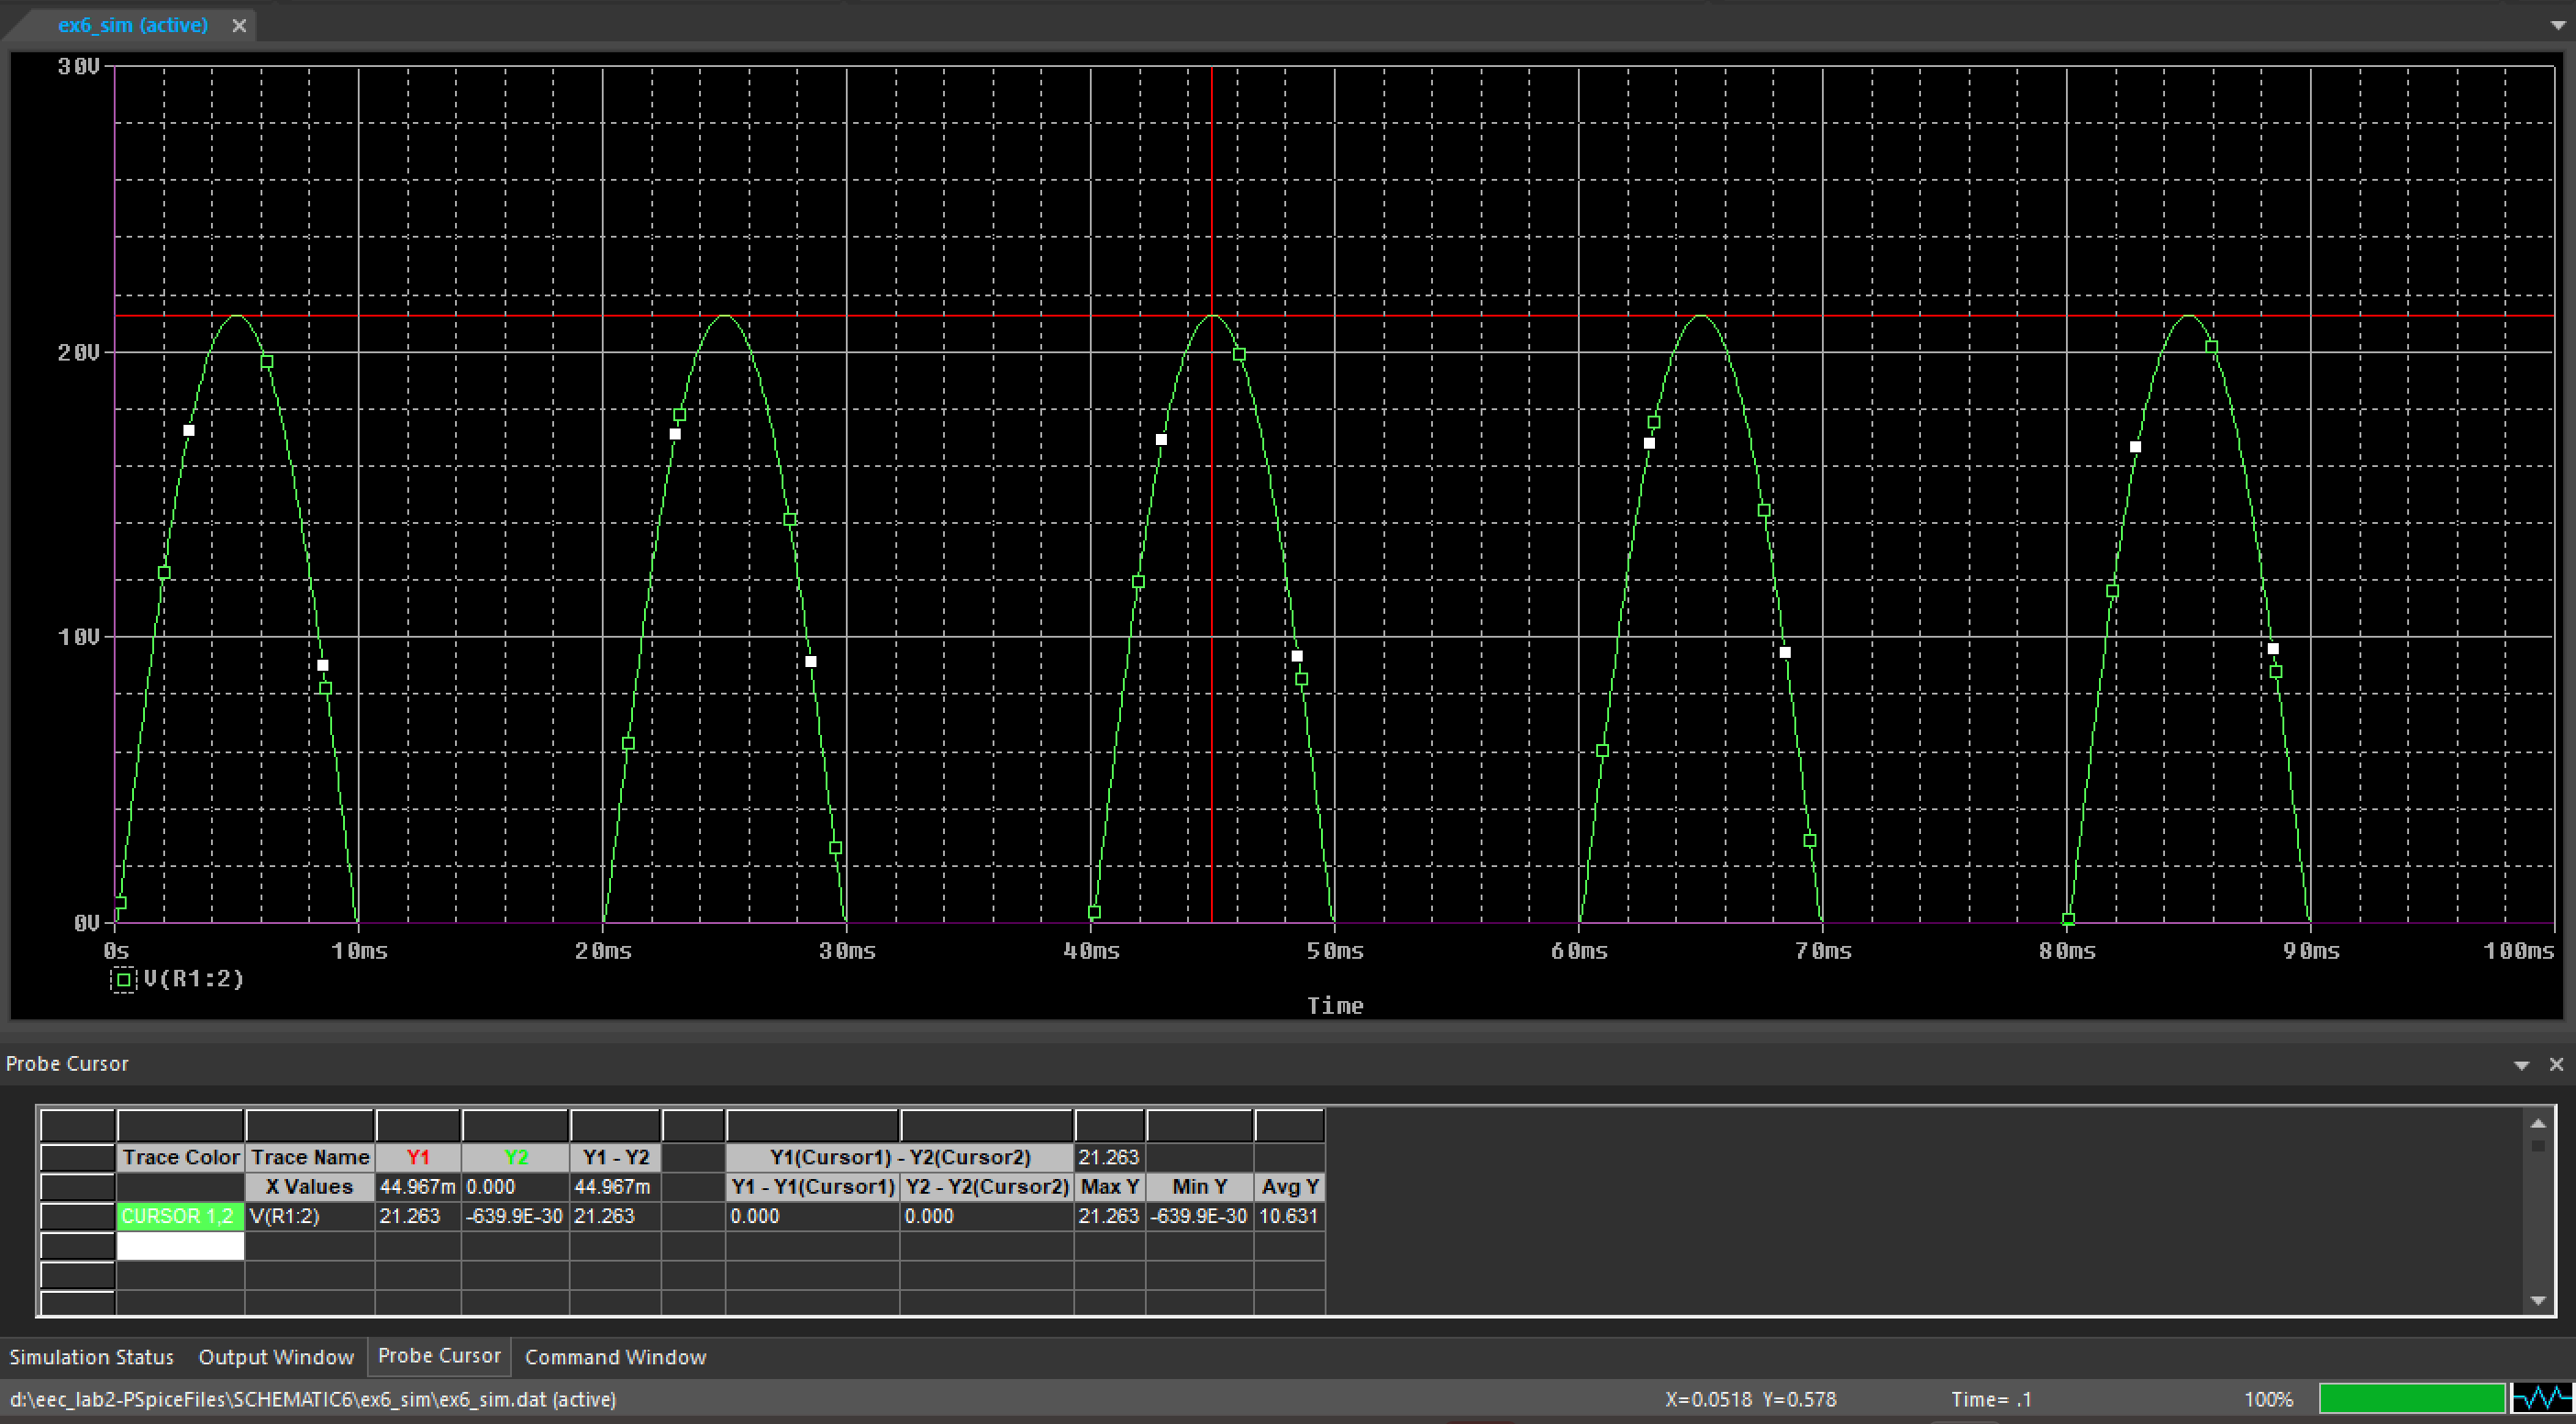
\includegraphics[width = 5in]{source/picture/bai_2/ex6_plot.png}

    \label{lab02_ex031g}
\end{figure}
% Exercise 4: Full-wave Rectifier.
% Given the following circuit. Simulate circuit to understand more about Half-wave Rectifier Application of Diode.

% \begin{figure}[!htp]
%     \centering
%     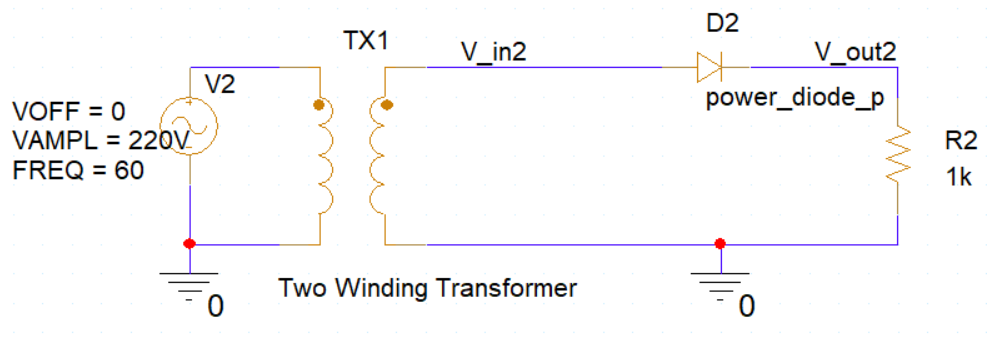
\includegraphics[width = 7cm]{source/picture/bai_2/Lab02_Ex032_HalfwaveRectifierWithTransformer.png}
%     \caption{Half-wave Rectifier with Input V Sin Source and Transformer}
%     \label{lab02_ex032}
% \end{figure}
% \textbf{Tips:}\\
% \begin{itemize}
%     \item To place \textbf{ Transformer}, choose \textbf{Place > Pspice Components... > Model Application... > System Modules > Transformer}
%     \item Configure \textbf{Transformer} as \textbf{Two Winding}
% \end{itemize}

\subsection{Full-wave Rectifier}
The following circuit is known as a full-wave bridge diode rectifier. Given that the transformer has the ratio $N1/N2 = 10$. Write the voltage difference equation $V_{AB}$ and $V_{CD}$. After that, perform a time-domain (transient) analysis to check the equation you've written.

\begin{figure}[H]
    \centering
    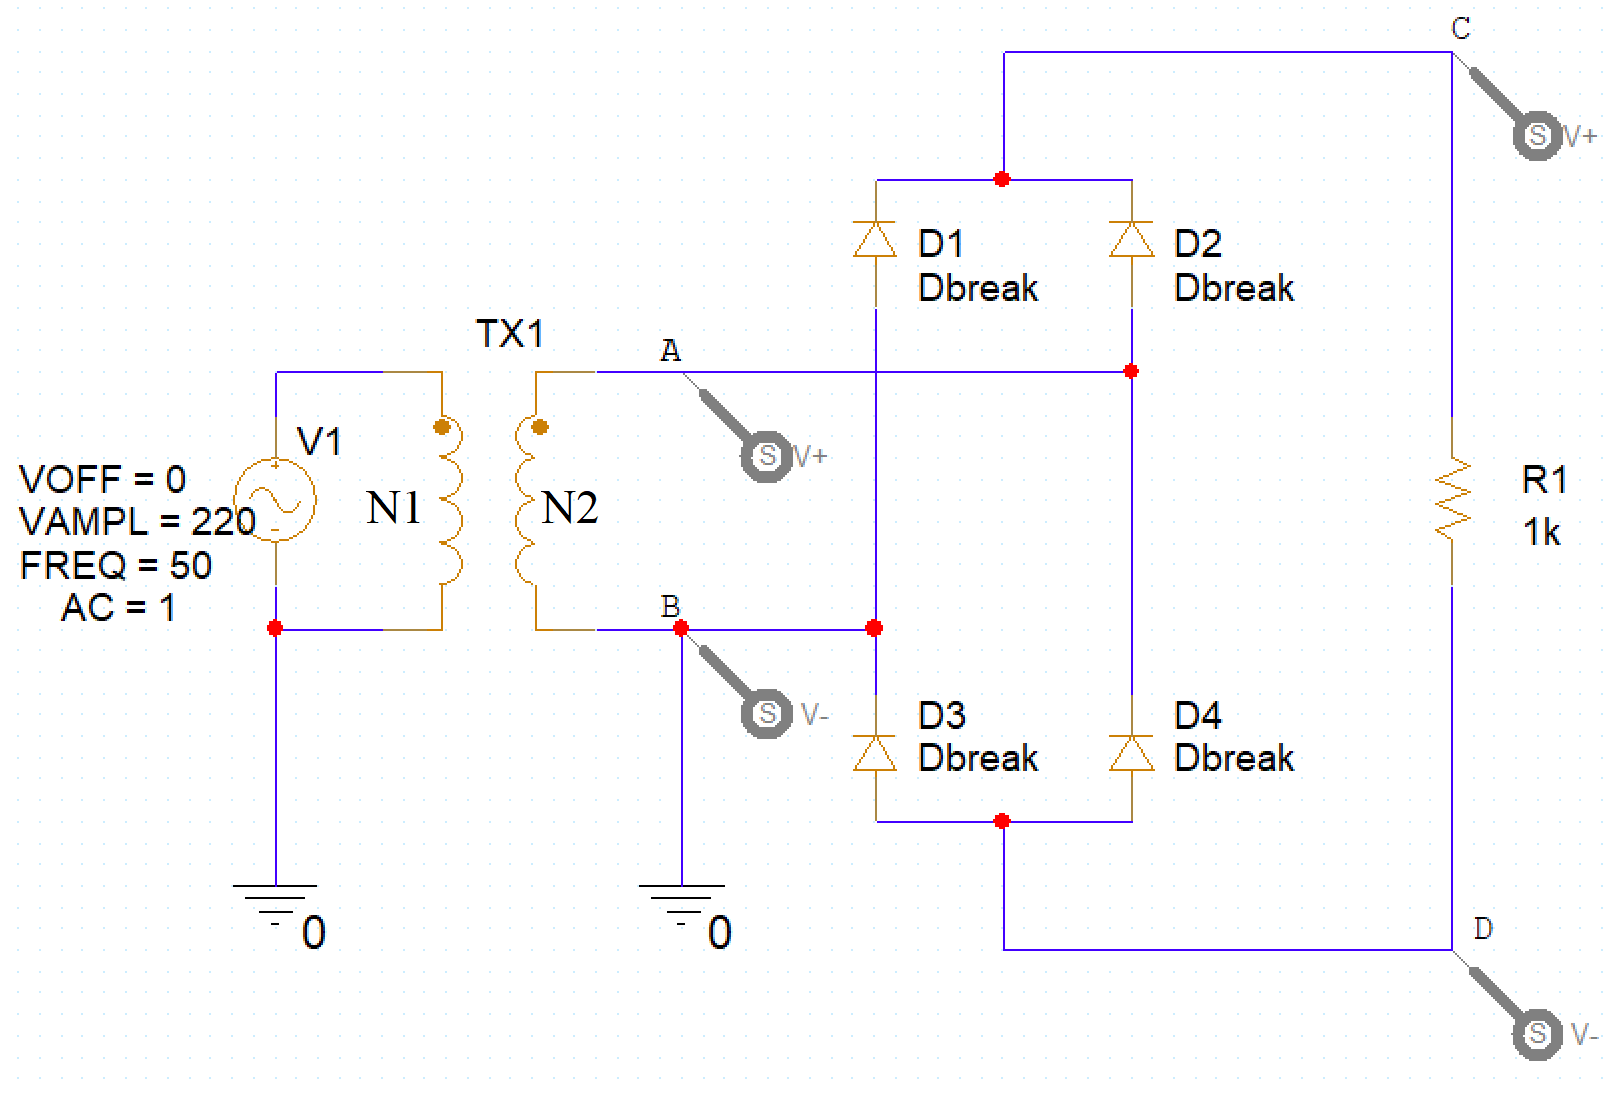
\includegraphics[width=5in]{source/picture/bai_2/LAB2_EX4_de.png}
    \caption{Full-wave bridge rectifier}
    \label{lab2_ex4_de}
\end{figure}

\textbf{\textit{Tips 1:}}
To place the component \textbf{transformer}:
\begin{itemize}
    \item \textbf{Step 1:} Go to \textbf{\textit{Place > PSpice Component > Modeling Application...}}
    \item \textbf{Step 2}: Browse for the \textbf{\textit{Transformer}} component under the \textbf{\textit{System Modules}} category as shown in the following Figure.
          \begin{figure}[H]
              \centering
              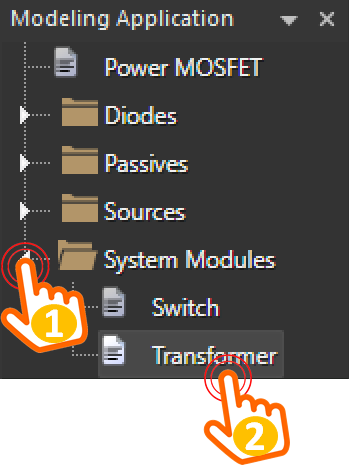
\includegraphics[width=5cm]{source/picture/bai_2/PSpicePlaceTransformer.png}
              \caption{Browse for the component \textbf{Transformer}}
              \label{pspicePlaceTransformer}
          \end{figure}
    \item \textbf{Step 3:} Set the transformation ratio before placing as shown below.
          \begin{figure}[H]
              \centering
              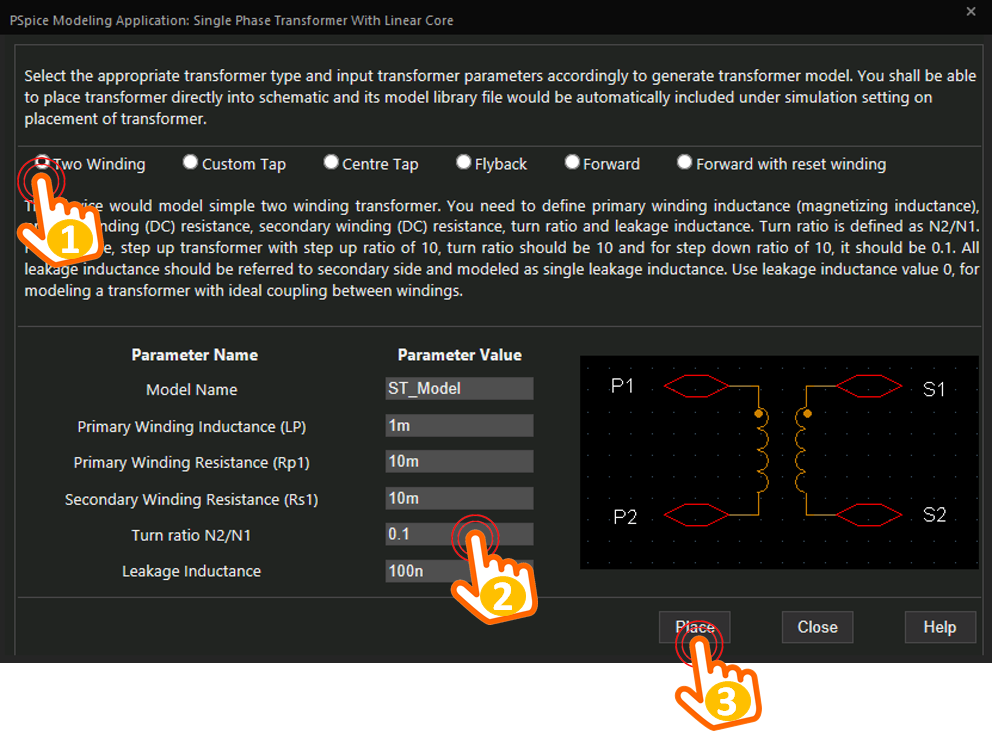
\includegraphics[width=15cm]{source/picture/bai_2/PSpiceTransformerSetting.png}
              \caption{Setting the transformation ratio before placing the transformer}
              \label{pspiceTransformerSetting}
          \end{figure}
\end{itemize}

\textbf{\textit{Tips 2:}}
The Voltage Differential Markers in PSPICE for TI:
\begin{figure}[H]
    \centering
    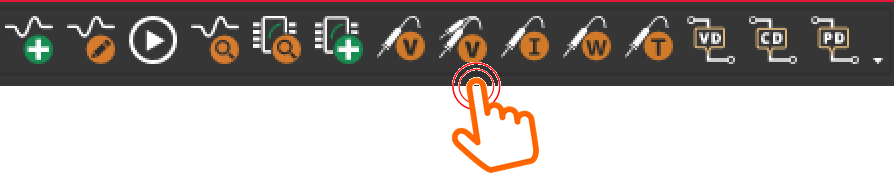
\includegraphics[width=12cm]{source/picture/bai_2/voltageDifferenceMarkers.png}
    \caption{The Voltage Differential Markers in PSPICE for TI}
    \label{vDiffMkrPair}
\end{figure}

\subsubsection{Theory calculation}
\textit{\textbf{Notes:}}\\

\textit{Explanations, formulas, and equations are expected rather than only results.}\\
\\
\textbf{\textit{Approximation:}} \textit{Diodes have $V_f$ = 0.7V}\bigskip\\
\\
$V_{AB} = V_1 \cdot \frac{N_2}{N_1} = V_1 \cdot 0.1$ \bigskip\\
According to Kirchoff's Voltage Law:\\
If $V_{AB}$ is on positive half cycle: $V_{CD} = V_{AB} - V_{D_2} - V_{D_3} = V_{AB} - 1.4$
\\
If $V_{AB}$ is on positive half cycle: $V_{CD} = V_{BA} - V_{D_1} - V_{D_4} = -V_{AB} - 1.4$
\\

$V_{CD} = |AB| - 1.4$ \bigskip\\


\subsubsection{Simulation}
The sinusoidal waveform of the voltage difference $V_{AB}$ has the period $T = $ \dotfill\\
If we want to perform the transient analysis in 10 periods of the waveform $V_{AB}$, the required time would be:\dotfill\\
If we want the sampling rate to be as ten times higher than the frequency of the sinusoidal voltage difference $V_{AB}$, the time interval between two consecutive sampling time points should be:\dotfill\bigskip\\
\\
Now, create a simulation profile as guided in the \textbf{Exercise \ref{halfwaveRectifier}} and perform your simulation to check it out!\\

\textbf{\textit{Simulation result:}}
Show both $V_{AB}$ and $V_{CD}$ in a single plot window to illustrate the relationship between them. Don't forget to use the cursors to prove that the equation you've written is correct.\\
\textit{(Your image(s) goes here)}\\
\begin{figure}[H]
    \centering
    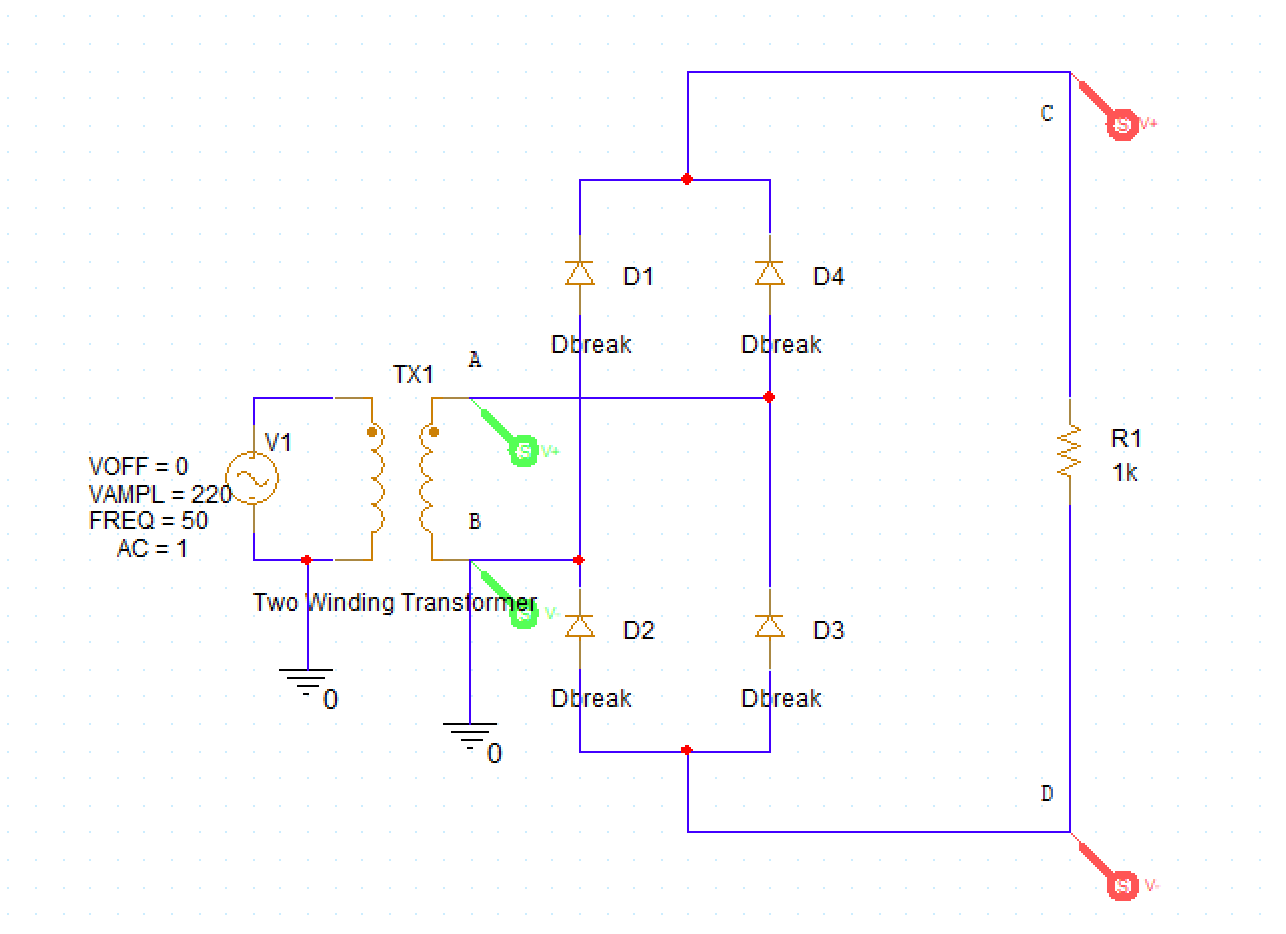
\includegraphics[width=500px]{source/picture/bai_2/ex7_sim.png}
\end{figure}

\begin{figure}[H]
    \centering
    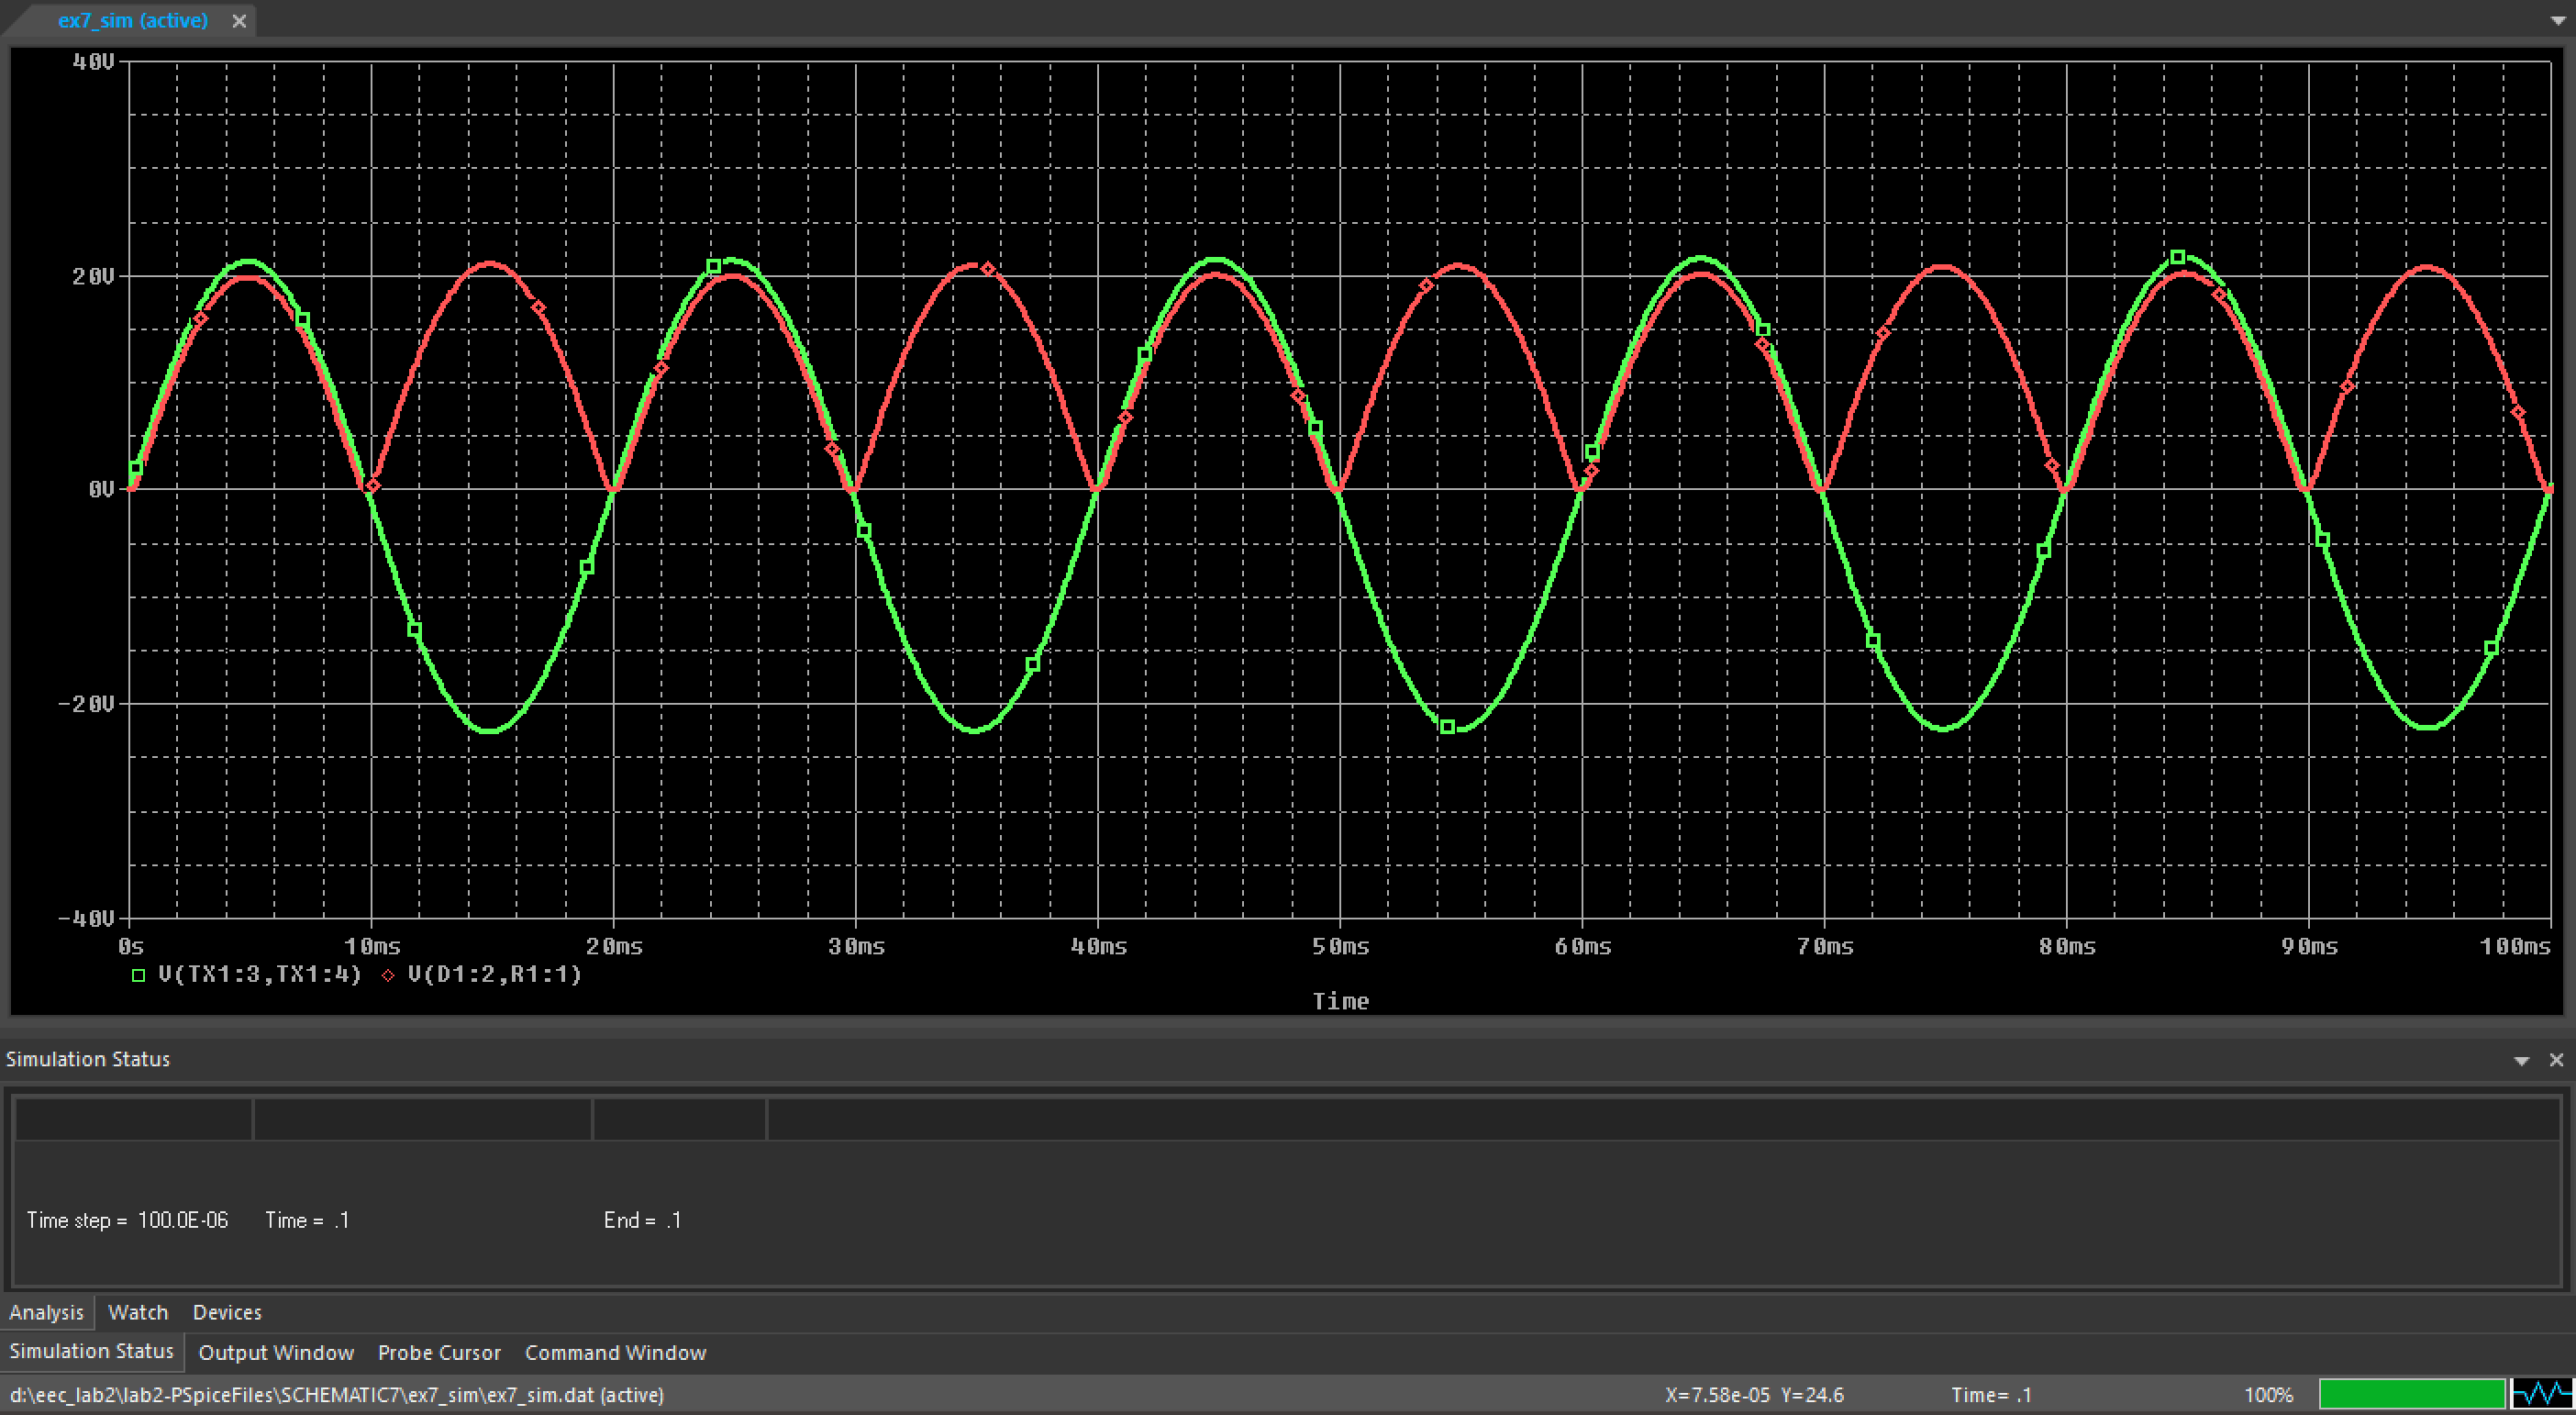
\includegraphics[width=500px]{source/picture/bai_2/ex7_plot.png}
\end{figure}
\newpage

\subsection{Zener Diode as a Regulator}
The Zener diode has a well-defined reverse-breakdown voltage, at which it starts conducting current, and continues operating continuously in the reverse-bias mode without getting damaged. Additionally, the voltage drop across the diode remains constant over a wide range of voltages, a feature that makes Zener diodes suitable for use in voltage regulation.

\begin{figure}[!htp]
    \centering
    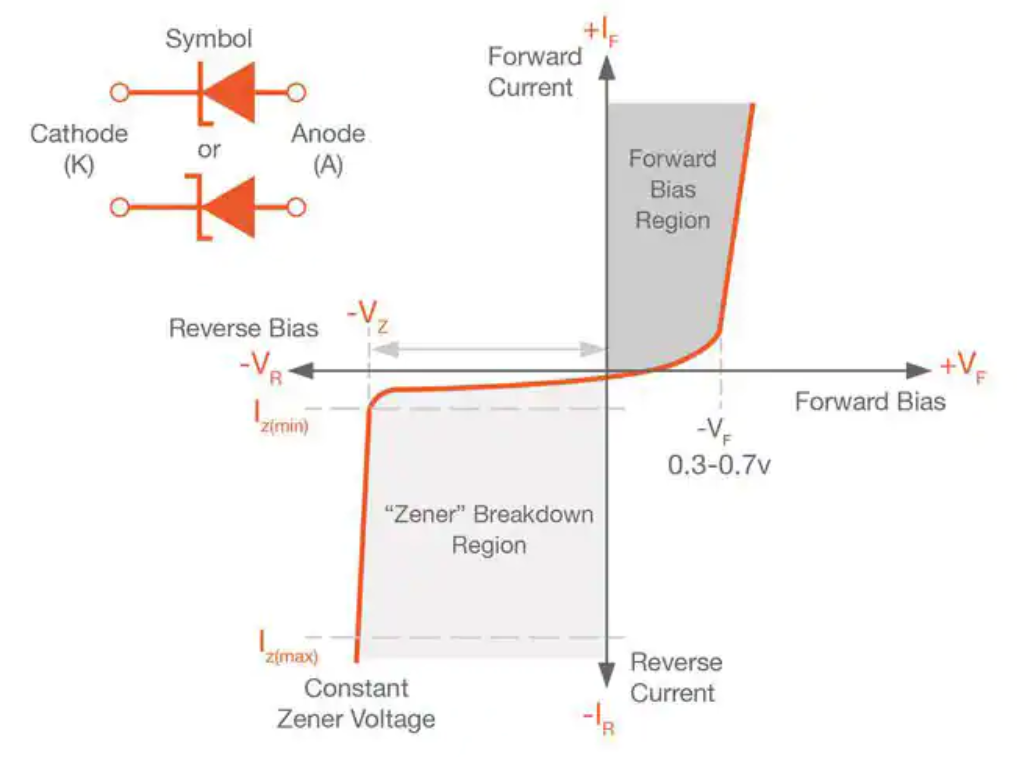
\includegraphics[width = 4in]{source/picture/bai_2/zener_3.PNG}
    \caption{Electrical characteristic of Zener diode}
    \label{lab02_zener1}
\end{figure}

In this exercise, a Zener diode is used to design a voltage regular circuit. The schematic in this exercise is given following:

\begin{figure}[!htp]
    \centering
    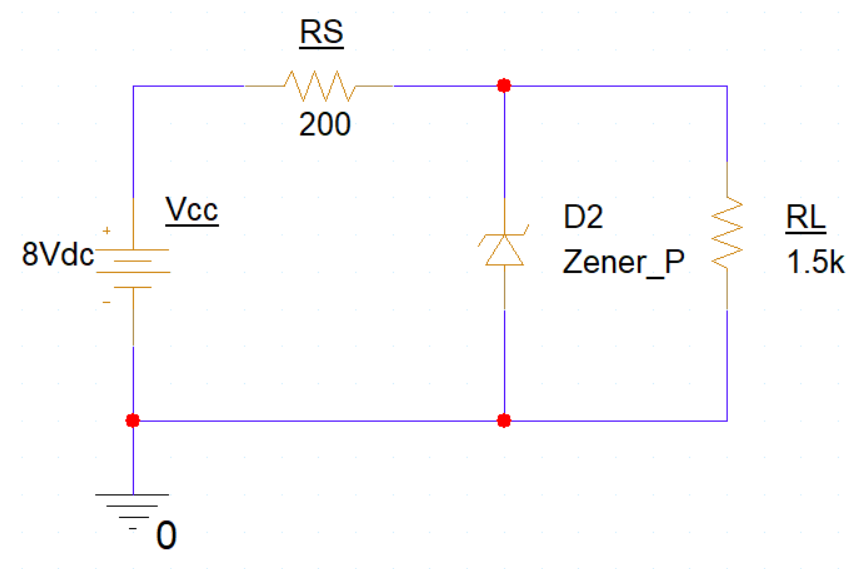
\includegraphics[width = 4in]{source/picture/bai_2/zener_1.PNG}
    \caption{Voltage regulator using Zener diode}
    \label{lab02_zener2}
\end{figure}

The Zener component in the circuit can be found in the Favourites list by search the keyword \textbf{Zener}. The full name of the component used in the circuit above is \textbf{Zenner\_P - Zener Diode (parameterized)}. The default Zener voltage of this component is $V_Z = 5V$. However, this value can be changed in the properties of the component (right click and select Edit Properties) for other simulations. \\

For theory calculation, students are supposed to provide equations for these values
\begin{itemize}
    \item $I_{L}$ = \dotfill\\
    \item $I_{S}$ = \dotfill\\
    \item $I_{Z}$ = \dotfill\\
    \item $P_{RS}$ = \dotfill\\
    \item $P_{Z}$ = \dotfill\\
\end{itemize}

Then, perform the calculation for the Zener diode voltage regulator with two different input voltage, including 8V and 12V power supply. Finally, run the simulations in PSpice (in \textbf{Bias Point} simulation profile) to confirm with the theory calculation. \\

The results are summarized in the table bellow.

\begin{center}
    \begin{tabular}{l|l|l|l|l|l|l|l|l|l|l|l|l|}
        \cline{2-13}
                                        & \multicolumn{6}{c|}{\textbf{Theory Calculation}} & \multicolumn{6}{c|}{\textbf{PSpice Simulation}}                                                                                                                                                      \\ \cline{2-13}
                                        & \multicolumn{1}{c|}{$I_S$}                       & \multicolumn{1}{c|}{$I_L$}                      & \multicolumn{1}{c|}{$I_Z$} & \multicolumn{1}{c|}{$V_L$} & \multicolumn{1}{c|}{$P_{RS}$} & $P_Z$ & $I_S$ & $I_L$ & $I_Z$ & $V_L$ & $P_{RS}$ & $P_Z$ \\ \hline
        \multicolumn{1}{|l|}{Vcc = 8V}  &                                                  &                                                 &                            &                            &                               &       &       &       &       &       &          &       \\ \hline
        \multicolumn{1}{|l|}{Vcc = 12V} &                                                  &                                                 &                            &                            &                               &       &       &       &       &       &          &       \\ \hline
    \end{tabular}
\end{center}

% % Exercise 5: Clipper Application.
% \subsection{Exercise 5: Clipper}
% Given the following circuit. Simulate circuit to understand more about Clipper Application of Diode.
% \begin{figure}[!htp]
%     \centering
%     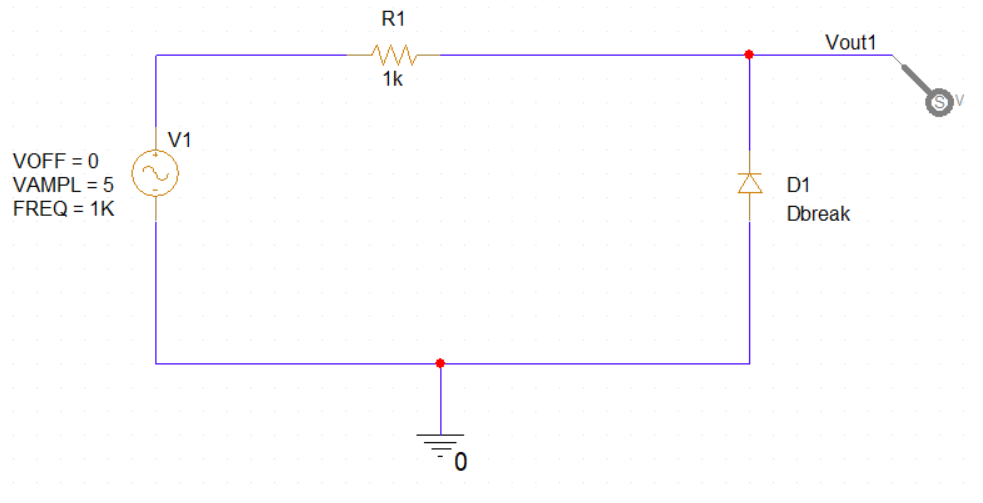
\includegraphics[width = 7cm]{source/picture/bai_2/Lab02_Ex05_Clipper_01.png}
%     \caption{Negative Peak Clipper}
%     \label{lab02_ex051}
% \end{figure}
% \begin{figure}[!htp]
%     \centering
%     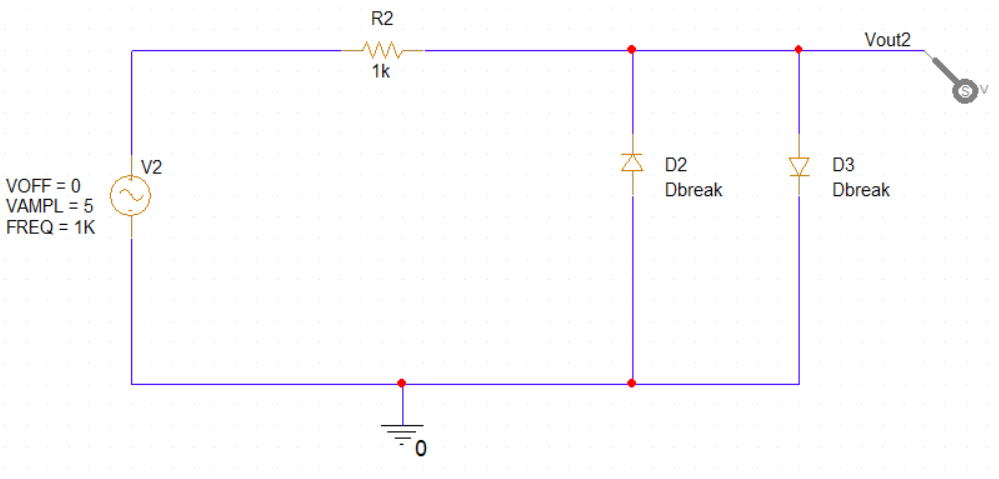
\includegraphics[width = 7cm]{source/picture/bai_2/Lab02_Ex05_Clipper_02.png}
%     \caption{Symmetrical Clipper}
%     \label{lab02_ex052}
% \end{figure}
% \begin{figure}[!htp]
%     \centering
%     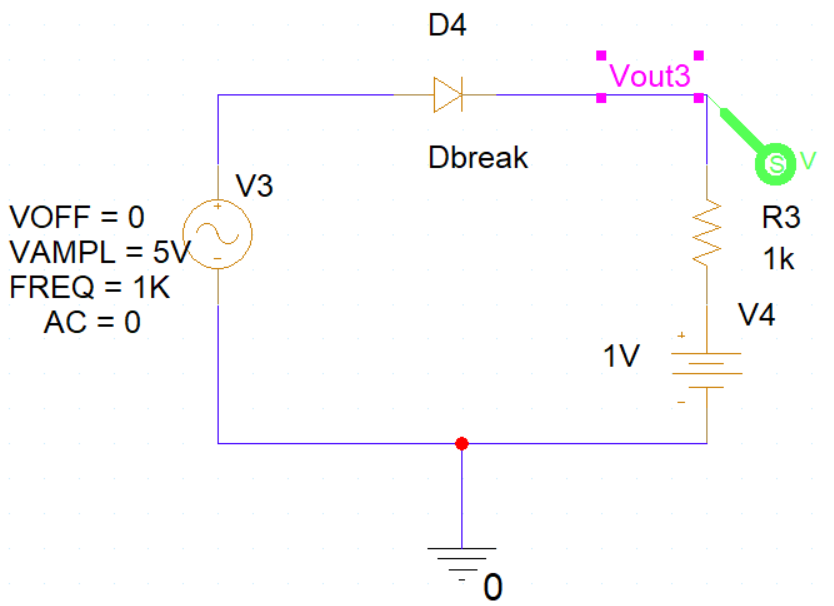
\includegraphics[width = 7cm]{source/picture/bai_2/Lab02_Ex05_Clipper_03.png}
%     \caption{Clipper with DC Source}
%     \label{lab02_ex053}
% \end{figure}

% \newpage
% \subsubsection{Calculation}
% \textit{\textbf{Notes:}}\\
% \textit{Explanations, formulas, and equations are expected rather than only results.}\\
% \\
% \textbf{\textit{Approximation:}} \textit{Diodes have $V_f$ = 0.7V and $r_d$ = 0 Ohm}\\
% \begin{itemize}
%     \item Minimum Value of $V_{out1}$ = \dotfill\\
%     \item Maximum Value of $V_{out1}$ = \dotfill\\
%     \item \textbf{Explanation} for value of \textbf{$V_{out1}$}: \dotfill\bigskip\\
%     \item Minimum Value of $V_{out2}$ = \dotfill\\
%     \item Maximum Value of $V_{out2}$ = \dotfill\\
%      \item \textbf{Explanation} for value of \textbf{$V_{out2}$}: \dotfill\bigskip\\
%     \item Minimum Value of $V_{out3}$ = \dotfill\\
%     \item Maximum Value of $V_{out4}$ = \dotfill\\  
%      \item \textbf{Explanation} for value of \textbf{$V_{out3}$}: \dotfill\bigskip\\
% \end{itemize}

% \textit{\textbf{Simulation results (check simulation values and images):}}
% \begin{itemize}
%     \item Minimum Value of $V_{out1}$ = \dotfill\\
%     \item Maximum Value of $V_{out1}$ = \dotfill\\
%     \item \textbf{Explanation} for value of \textbf{$V_{out1}$}: \dotfill\bigskip\\
%     \item Minimum Value of $V_{out2}$ = \dotfill\\
%     \item Maximum Value of $V_{out2}$ = \dotfill\\
%      \item \textbf{Explanation} for value of \textbf{$V_{out2}$}: \dotfill\bigskip\\
%     \item Minimum Value of $V_{out3}$ = \dotfill\\
%     \item Maximum Value of $V_{out4}$ = \dotfill\\  
%      \item \textbf{Explanation} for value of \textbf{$V_{out3}$}: \dotfill\bigskip\\
% \end{itemize}

% \textbf{Simulation Images}\\
% Diagrams \textbf{Time Domain (Transient)} to display relationship between input voltage and output voltage for each circuit.

% % Exercise 6: Clampers Application.
% \subsection{Exercise 6: Clamper Application}
% Given the following circuit. Simulate circuit to understand more about Clampers Application of Diode.
% \begin{figure}[!htp]
%     \centering
%     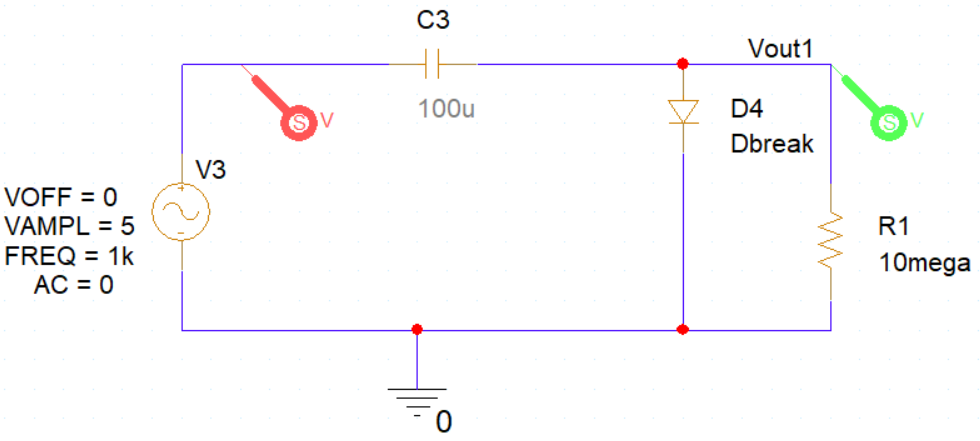
\includegraphics[width = 7cm]{source/picture/bai_2/Lab02_Ex061.png}
%     \caption{Positive Clamper}
%     \label{lab02_ex061}
% \end{figure}
% \begin{figure}[!htp]
%     \centering
%     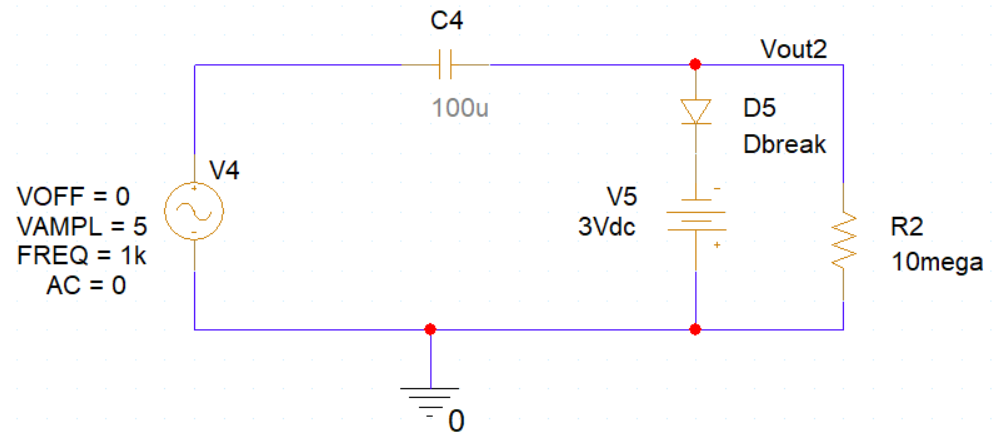
\includegraphics[width = 7cm]{source/picture/bai_2/Lab02_Ex062.png}
%     \caption{Positive Clamper with Source DC 3Vdc}
%     \label{lab02_ex062}
% \end{figure}
% \begin{figure}[!htp]
%     \centering
%     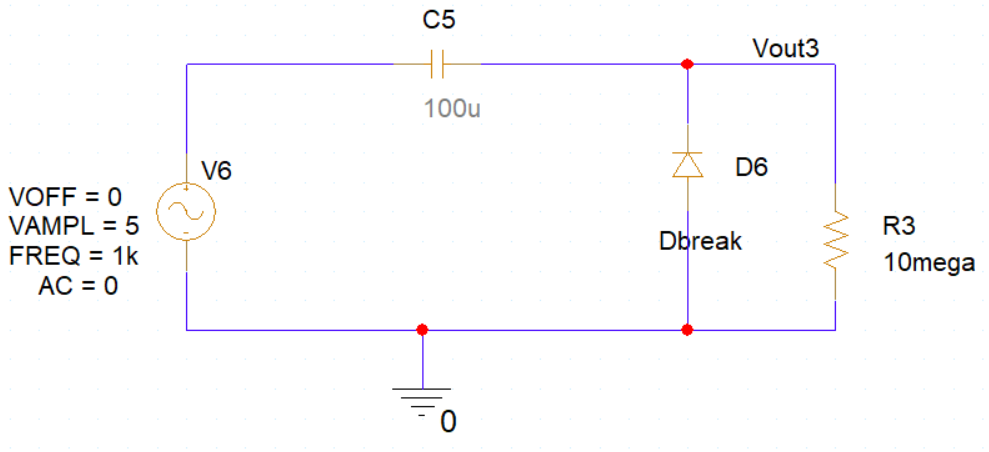
\includegraphics[width = 7cm]{source/picture/bai_2/Lab02_Ex063.png}
%     \caption{Negative Clamper}
%     \label{lab02_ex063}
% \end{figure}
% \begin{figure}[!htp]
%     \centering
%     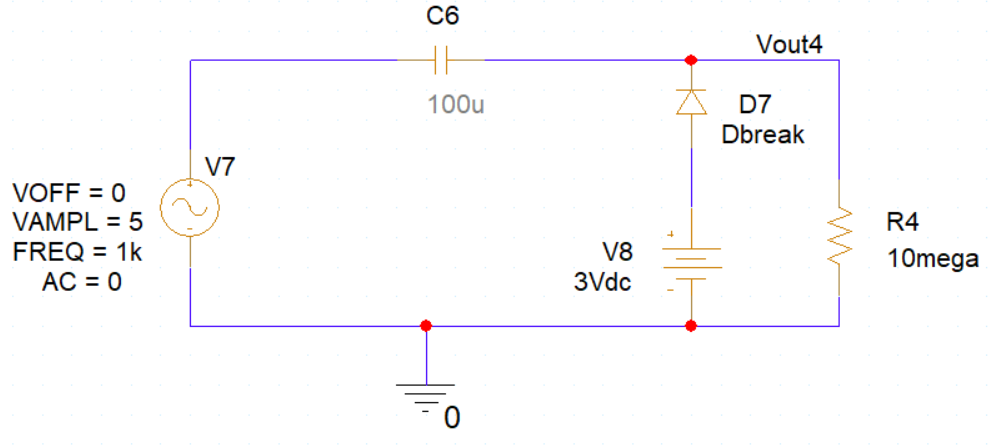
\includegraphics[width = 7cm]{source/picture/bai_2/Lab02_Ex064.png}
%     \caption{Nagative Clamper with Source DC 3Vdc}
%     \label{lab02_ex064}
% \end{figure}

% \subsubsection{Calculation and Explanation}
% \textit{\textbf{Notes:}}\\
% \textit{Explanations, formulas, and equations are expected rather than only results.}\\
% \textbf{Approximation: }: Diodes have $V_f$ = 0.7V and $r_d$ = 0 Ohm\\

% \textbf{Simulation Images}\\
% Diagrams \textbf{Time Domain (Transient)} to display relationship between input voltage and output voltage for each circuit.
% \begin{itemize}
%     \item Capture simulation diagram for each circuit
%     \item \textbf{Analyze} briefly circuit (for each diagram) 
% \end{itemize}
% Exercise 7: AC/DC Power Circuit Application.
\subsection{AC/DC Power Circuit Application}
In this exercise, we are building step by step an AC to DC voltage source transformation circuit. Students perform a time-domain simulation and write out comments and explanations for each step.\\
\\
\textbf{\textit{Tips: }} To place a capacitor, go to \textbf{\textit{Place > PSpice Component > Capacitor}}

\begin{itemize}
    \item \textbf{Step 1:} The rectified voltage without any filtering or being regulated.
          \begin{figure}[H]
              \centering
              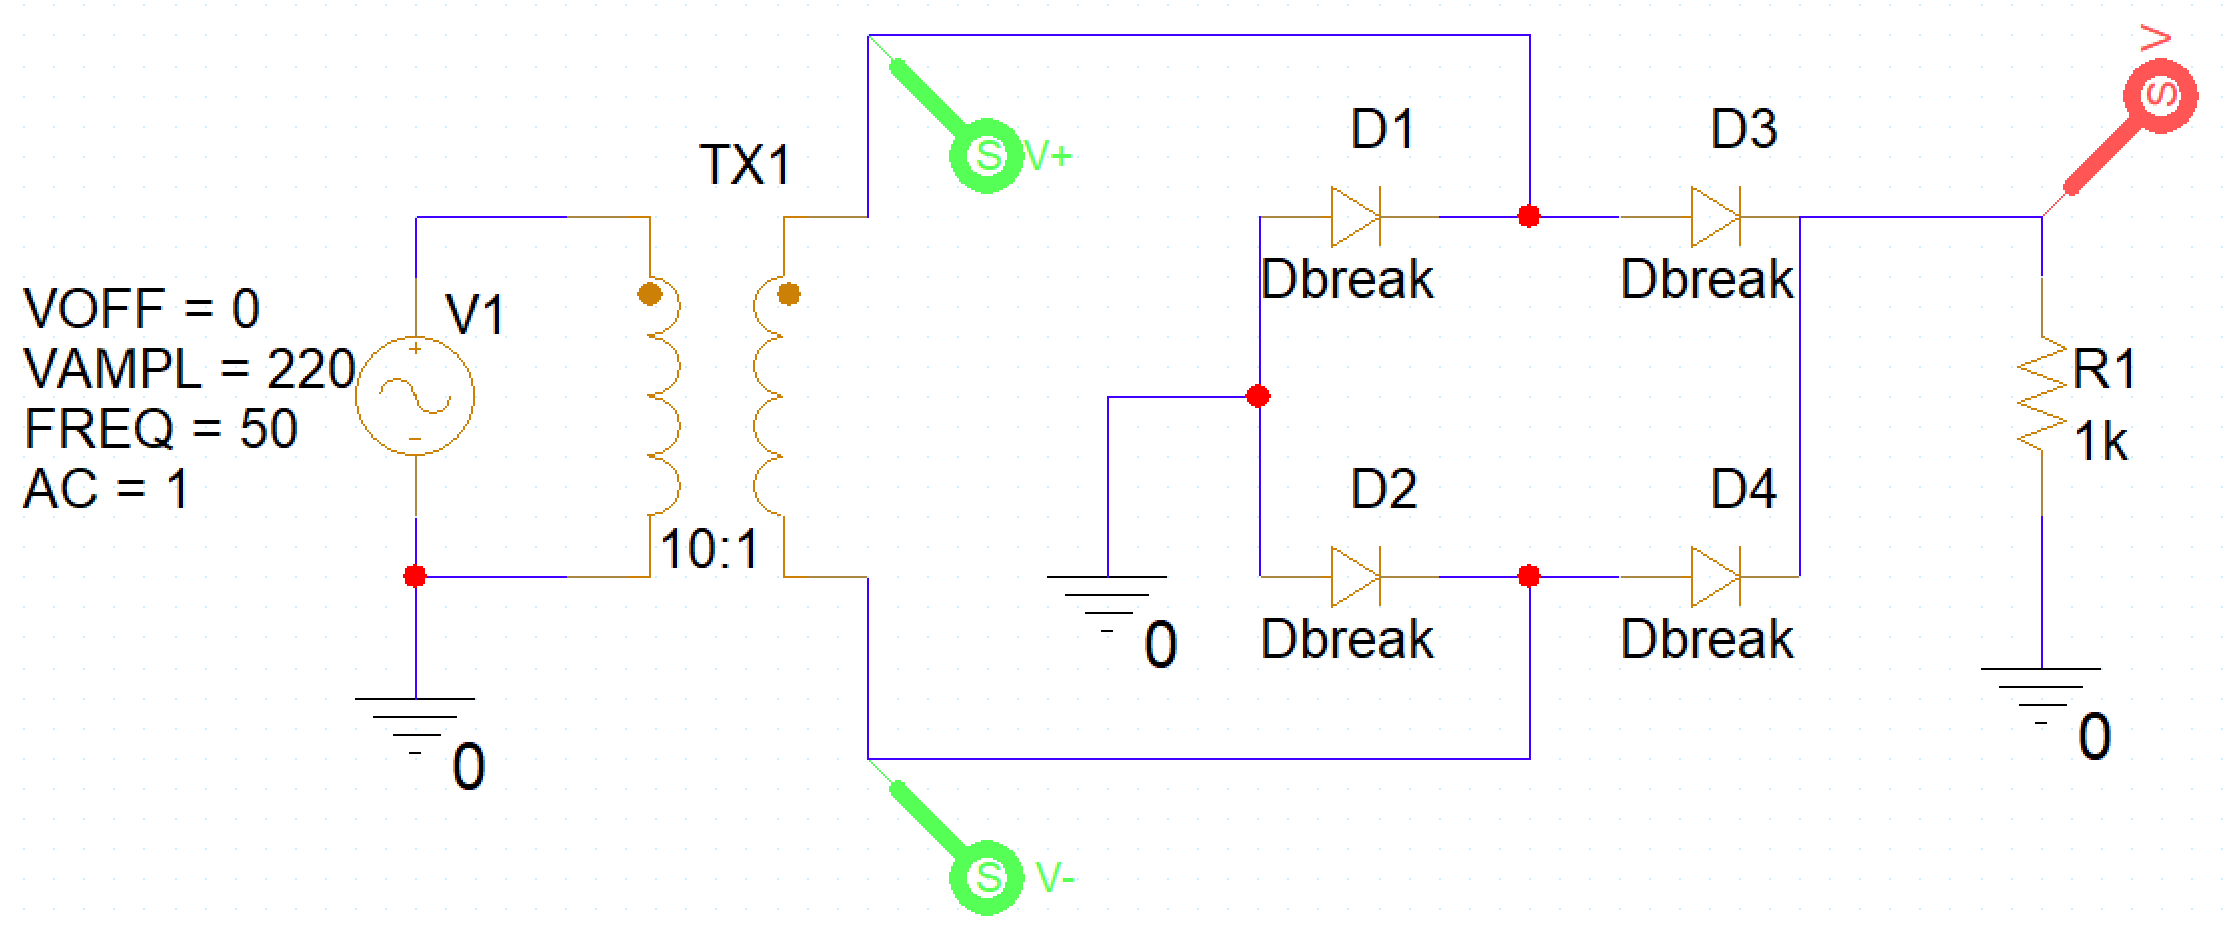
\includegraphics[width=\linewidth]{source/content/lab2_ex9_step1.png}
              \caption{The rectified voltage without any filtering or being regulated}
              \label{lab2_ex9_step1}
          \end{figure}
          \textit{\textbf{Simulation result:}} \textit{Your image goes here}\\
          \\
          \vspace{8cm}
          \\
          \textbf{\textit{Any comments or explanations:}}
          \dotfill\bigskip\par\mbox{}\dotfill
          \dotfill\bigskip\par\mbox{}\dotfill
          \dotfill\bigskip\par\mbox{}\dotfill
          \dotfill\bigskip\par\mbox{}\dotfill
          \dotfill\bigskip\par\mbox{}\dotfill
          \dotfill\bigskip\par\mbox{}\dotfill

    \item \textbf{Step 2:} Rectified voltage regulated with a $10\micro F$ capacitor.
          \begin{figure}[H]
              \centering
              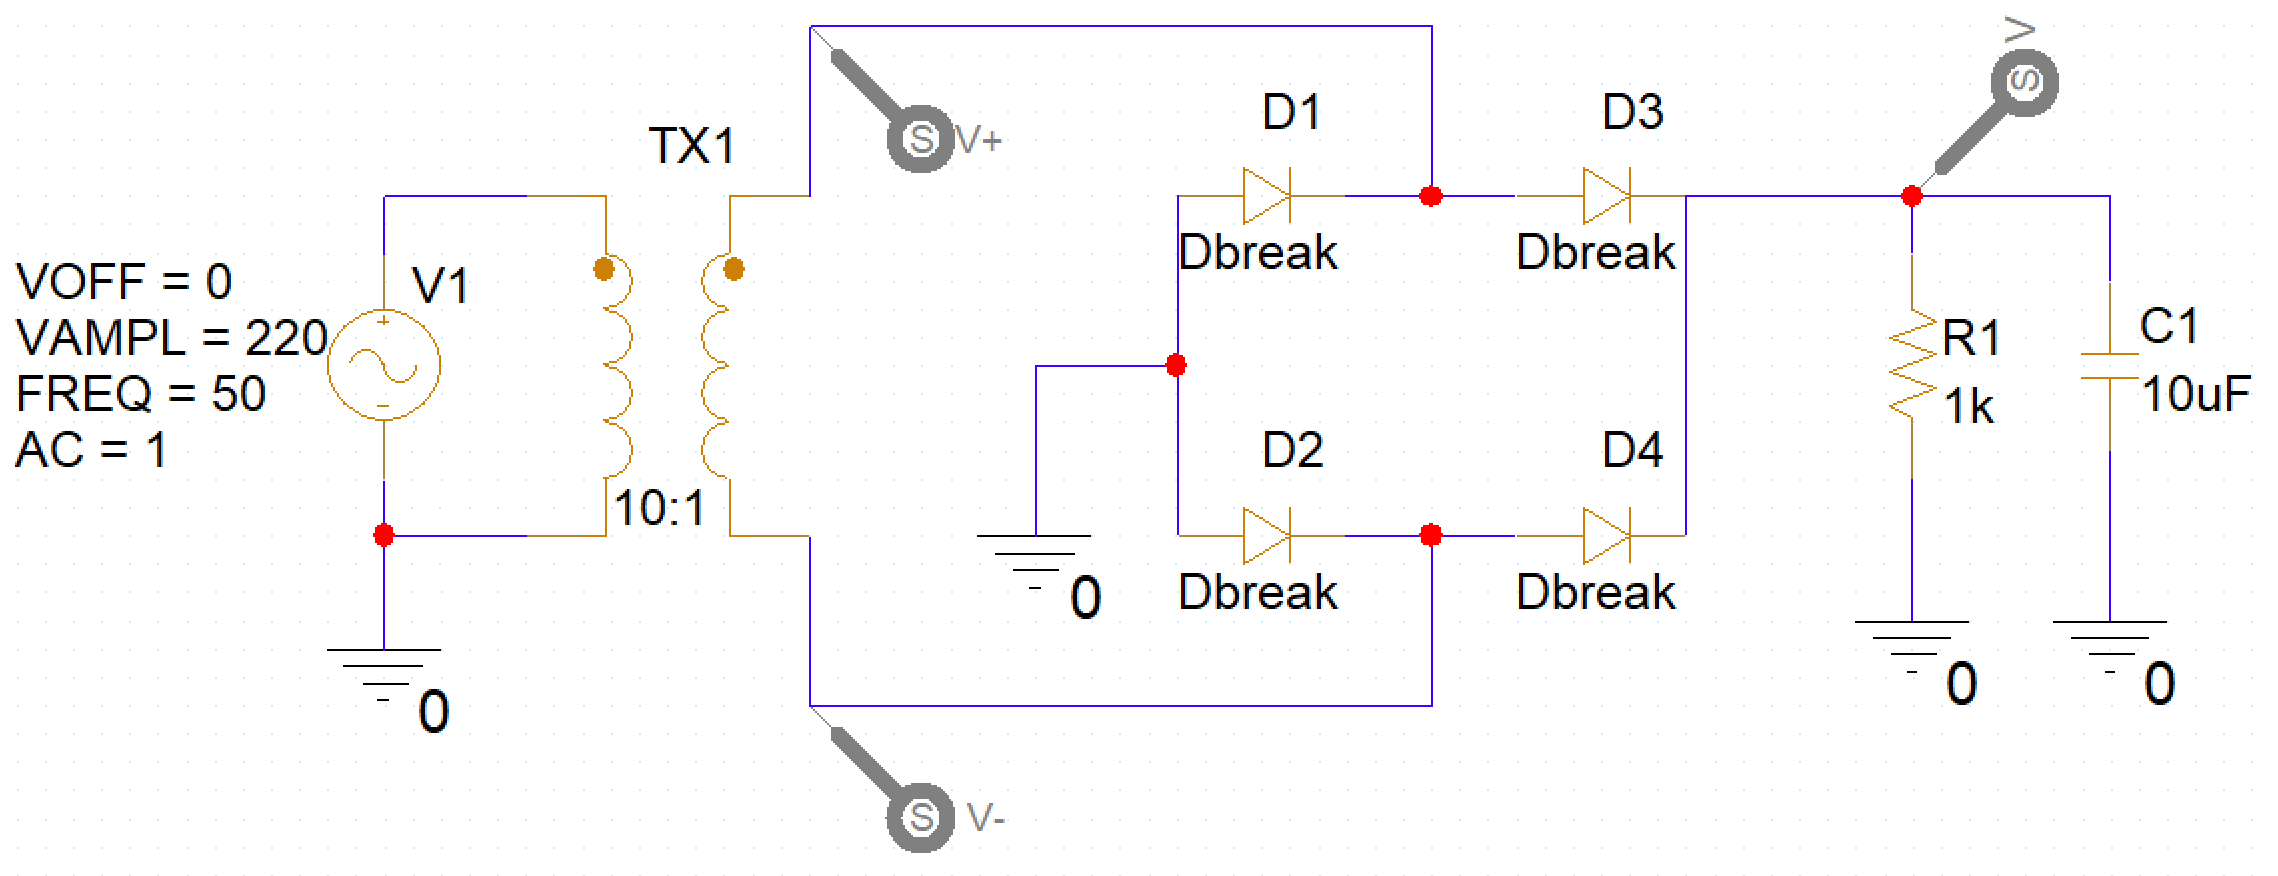
\includegraphics[width=\linewidth]{source/content/lab2_ex9_step2.png}
              \caption{Rectified voltage regulated with a capacitor}
              \label{lab2_ex9_step2}
          \end{figure}
          \textit{\textbf{Simulation result(s):}} \textit{Your image goes here}\\
          \\
          \vspace{8cm}
          \\
          \textbf{\textit{Any comments or explanations:}}
          \dotfill\bigskip\par\mbox{}\dotfill
          \dotfill\bigskip\par\mbox{}\dotfill
          \dotfill\bigskip\par\mbox{}\dotfill
          \dotfill\bigskip\par\mbox{}\dotfill
          \dotfill\bigskip\par\mbox{}\dotfill
          \dotfill\bigskip\par\mbox{}\dotfill
    \item \textbf{Step 3}: Replace the $10\micro F$ capacitor with a $680\micro F$ one and re-run the simulation, recognize the change in the result and explain.\\
          \textit{\textbf{Simulation result(s):}} \textit{Your image goes here}\\
          \\
          \vspace{6cm}
          \\
          \textbf{\textit{Any comments or explanations:}}
          \dotfill\bigskip\par\mbox{}\dotfill
          \dotfill\bigskip\par\mbox{}\dotfill
          \dotfill\bigskip\par\mbox{}\dotfill
          \dotfill\bigskip\par\mbox{}\dotfill
          \dotfill\bigskip\par\mbox{}\dotfill
          \dotfill\bigskip\par\mbox{}\dotfill
    \item \textbf{Step 4:} Add a zener diode as in Figure \ref{lab2_ex9_step3} with the $zener voltage$ properties set to 22 volt then simulate the circuit and comment or explain the result.
          \begin{figure}[H]
              \centering
              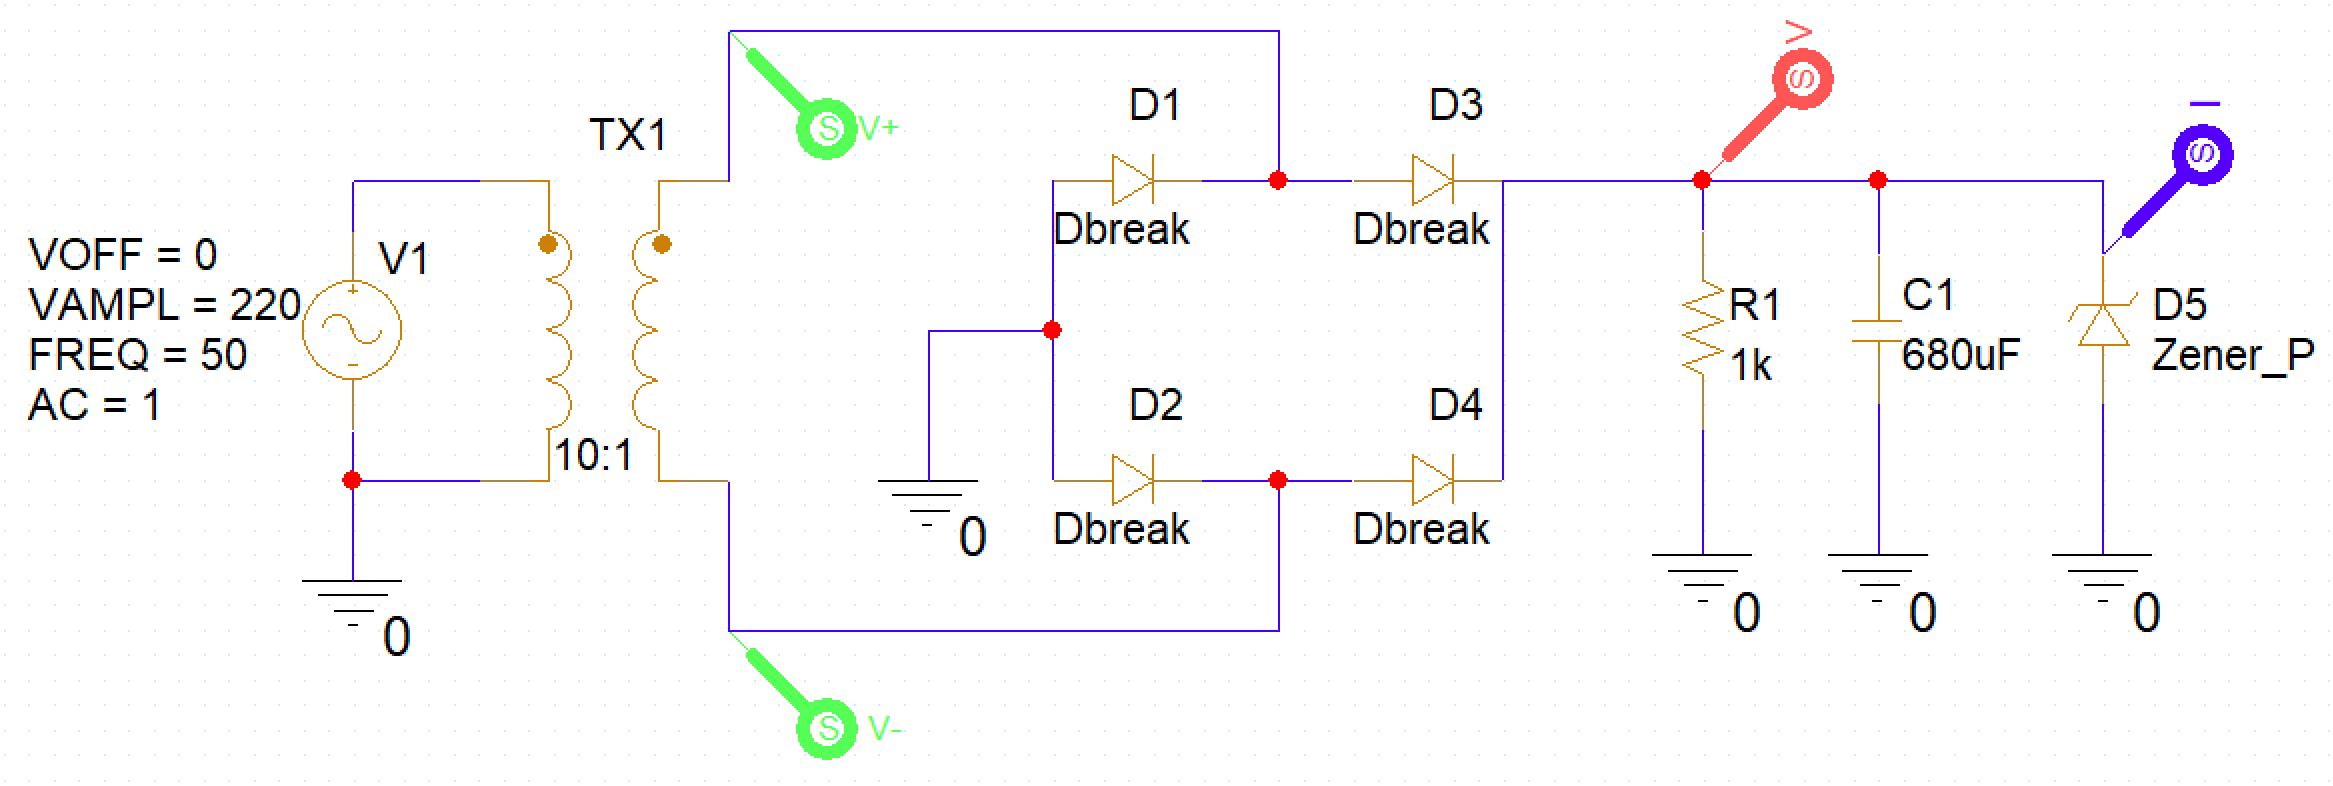
\includegraphics[width=\linewidth]{source/content/lab2_ex9_step3.png}
              \caption{Rectified voltage regulated with a capacitor and a zener diode}
              \label{lab2_ex9_step3}
          \end{figure}
          \textit{\textbf{Simulation result(s):}} \textit{Your image goes here}\\
          \\
          \vspace{8cm}
          \\
          \textbf{\textit{Any comments or explanations:}}
          \dotfill\bigskip\par\mbox{}\dotfill
          \dotfill\bigskip\par\mbox{}\dotfill
          \dotfill\bigskip\par\mbox{}\dotfill
          \dotfill\bigskip\par\mbox{}\dotfill
          \dotfill\bigskip\par\mbox{}\dotfill
          \dotfill\bigskip\par\mbox{}\dotfill
    \item \textbf{Step 5:} Change the $zener voltage$ properties of the zener diode to 20 voltage and then re-run the simulation. Comment and explain any changes in the result.\\
          \textit{\textbf{Simulation result(s):}} \textit{Your image goes here}\\
          \\
          \vspace{8cm}
          \\
          \textbf{\textit{Any comments or explanations:}}
          \dotfill\bigskip\par\mbox{}\dotfill
          \dotfill\bigskip\par\mbox{}\dotfill
          \dotfill\bigskip\par\mbox{}\dotfill
          \dotfill\bigskip\par\mbox{}\dotfill
          \dotfill\bigskip\par\mbox{}\dotfill
          \dotfill\bigskip\par\mbox{}\dotfill
\end{itemize}

\newpage

% AC/DC Power Circuit Application With LM2596_12P0_TRANS
\subsection{Exercise 8:  AC/DC Power Circuit Application With LM2596\_5P0\_TRANS}
Figure \ref{incomplete2596} describes an incomplete Texas Instrument LM2596 - 5.0 Switching Power Supply circuit. It lacks a Zener diode voltage regulator and an inductor reducing the voltage variation. At first, let perform a time-domain (transient) simulation with this incomplete circuit and figure out the problem with the output voltage (the voltage marker at R1).

\begin{figure}[H]
    \centering
    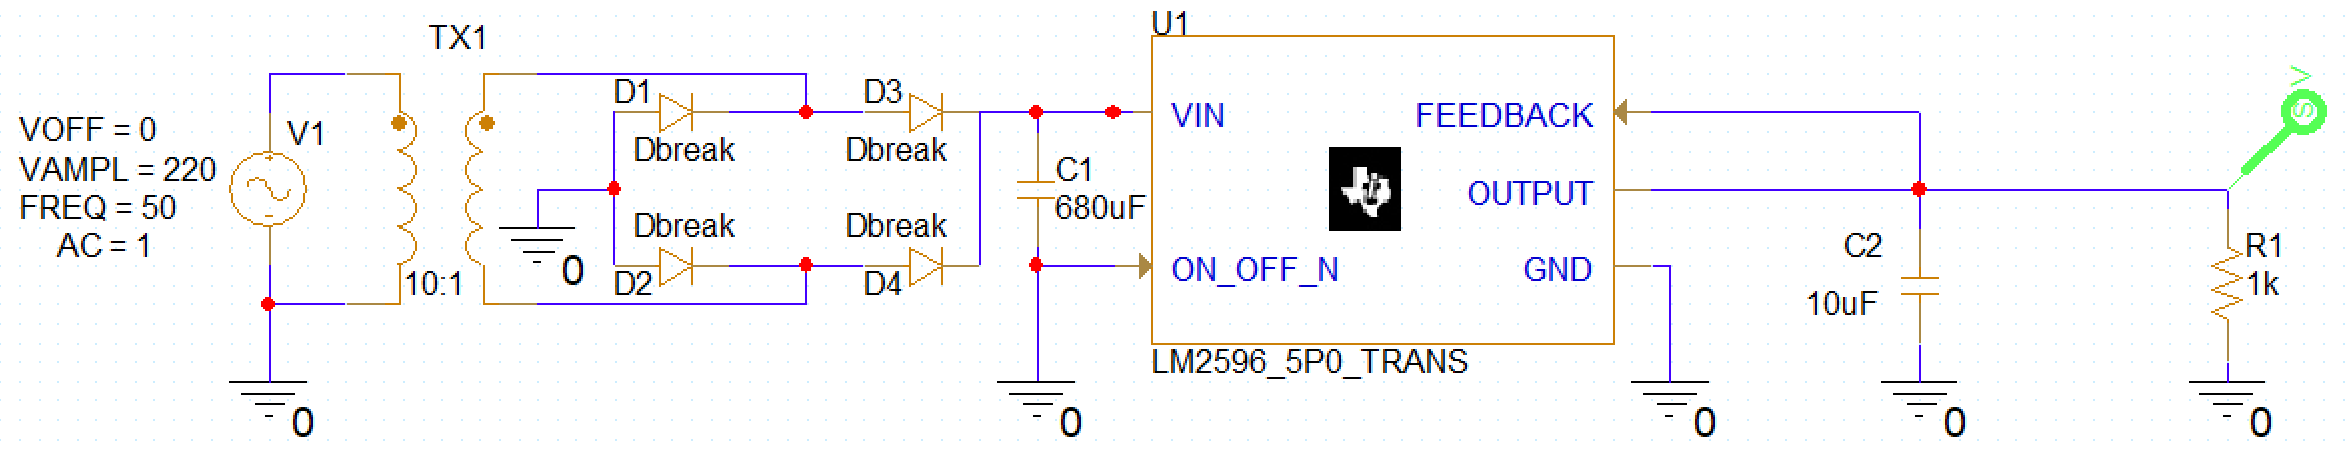
\includegraphics[width=18cm]{source/picture/bai_2/lab2_ex10_step1.png}
    \caption{Incomplete switching power supply circuit}
    \label{incomplete2596}
\end{figure}

\textbf{\textit{Tips:}}\\
\\
To place the switching power supply IC LM2596 - 5.0, go to \textbf{\textit{Place > PSpice Component... > Search...}} then search for \textit{LM2596\_5P0\_TRANS}.

But before you can perform a transient simulation and analysis with this circuit, we will need to pay attention to some minor settings on the simulation profile.\\
\\
\begin{figure}[H]
    \centering
    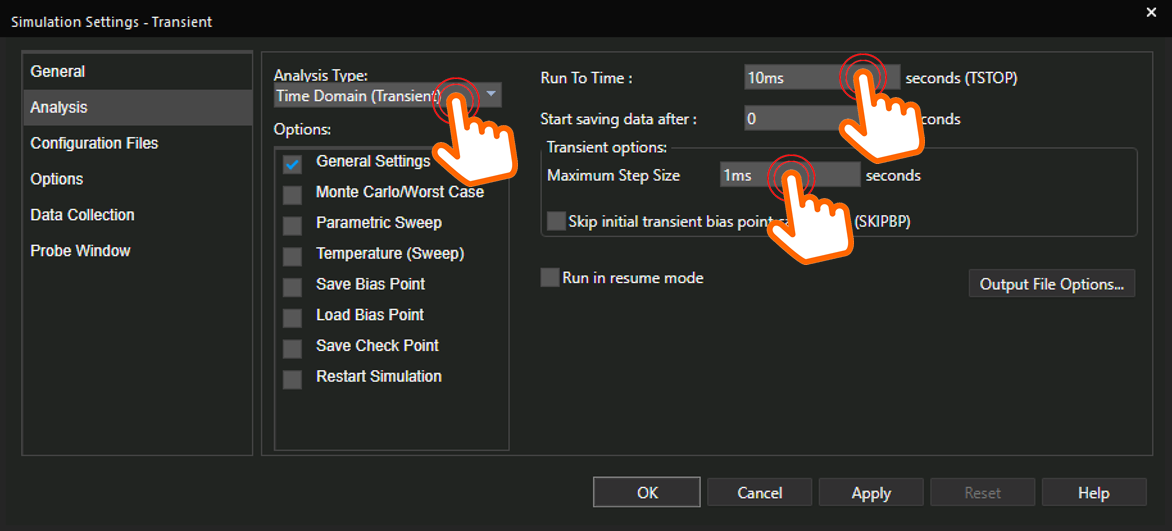
\includegraphics[width=\linewidth]{source/picture/bai_2/lab2_ex10_simProf1.png}
    \caption{Set the transient simulation duration}
    \label{lab2_ex10_simProf1}
\end{figure}

\begin{figure}[H]
    \centering
    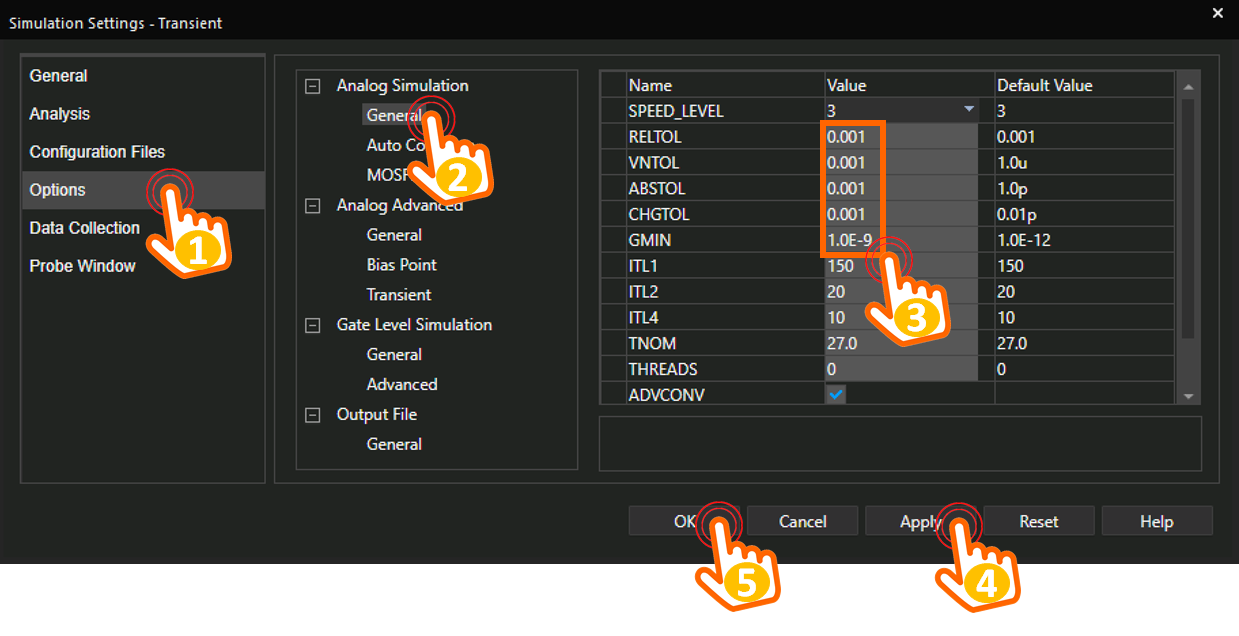
\includegraphics[width=\linewidth]{source/picture/bai_2/lab2_ex10_simProf2.png}
    \caption{Set the transient calculation accuracy}
    \label{lab2_ex10_simProf2}
\end{figure}

\textit{\textbf{Simulation result(s):}} \textit{Your image goes here}\\
\\
\vspace{8cm}
\\
\textbf{\textit{Any comments or explanations:}}
\dotfill\bigskip\par\mbox{}\dotfill
\dotfill\bigskip\par\mbox{}\dotfill
\dotfill\bigskip\par\mbox{}\dotfill
\dotfill\bigskip\par\mbox{}\dotfill
\dotfill\bigskip\par\mbox{}\dotfill
\dotfill\bigskip\par\mbox{}\dotfill
\\
\\
Next, add an inductor $33\micro H$ to the circuit as shown in Figure \ref{lab2_ex10_step2} then re-run the simulation and explain any improvements.
\begin{figure}[H]
    \centering
    \includegraphics[width=18cm]{source/picture/bai_2/lab2_ex10_step2.png}
    \caption{A $33\micro H$ inductor added to the circuit}
    \label{lab2_ex10_step2}
\end{figure}

\textit{\textbf{Simulation result(s):}} \textit{Your image goes here}\\
\\
\vspace{8cm}
\\
\textbf{\textit{Any comments or explanations:}}
\dotfill\bigskip\par\mbox{}\dotfill
\dotfill\bigskip\par\mbox{}\dotfill
\dotfill\bigskip\par\mbox{}\dotfill
\dotfill\bigskip\par\mbox{}\dotfill
\dotfill\bigskip\par\mbox{}\dotfill
\dotfill\bigskip\par\mbox{}\dotfill
\\
\\
Continue, add a 5V Zener diode to the circuit as shown in Figure \ref{lab2_ex10_step3}, change the capacitor to $220\micro F$, add a current marker to the Zener diode, re-run the simulation and explain the role of the Zener diode in the circuit.
\begin{figure}[H]
    \centering
    \includegraphics[width=17cm]{source/picture/bai_2/lab2_ex10_step3.png}
    \caption{A 5V Zener diode added to the circuit}
    \label{lab2_ex10_step3}
\end{figure}

\textit{\textbf{Simulation result(s):}} \textit{Your image goes here}\\
\\
\vspace{8cm}
\\
\textbf{\textit{Any comments or explanations:}}
\dotfill\bigskip\par\mbox{}\dotfill
\dotfill\bigskip\par\mbox{}\dotfill
\dotfill\bigskip\par\mbox{}\dotfill
\dotfill\bigskip\par\mbox{}\dotfill
\dotfill\bigskip\par\mbox{}\dotfill
\dotfill\bigskip\par\mbox{}\dotfill
\\
\\

